\documentclass{article}

\usepackage[margin=2.5cm,left=2cm,includefoot]{geometry}
\usepackage{graphicx}
\usepackage{float}
\usepackage[space]{grffile}
\usepackage{hyperref}
\usepackage[export]{adjustbox}
\usepackage{multicol}

% Header and footer
\usepackage{fancyhdr}
\pagestyle{fancy}

\rhead{COS301 - \LaTeX}
\lhead{Team Charlie}
\fancyfoot{}
\fancyfoot[R]{Page \thepage}

\renewcommand{\headrulewidth}{2pt}
\renewcommand{\footrulewidth}{1pt}
%

\begin{document}

	\begin{titlepage}
		\begin{center}
		
			\line(1,0){300}\\
			[6mm]
			\huge{
				\bfseries Software Requirements Specification\\
				and\\
				Technology Neutral Process Design
			}\\
			[2mm]
			\line(1,0){200}\\
			[15mm]
			\textsc{\large P.A.P.E.R.S (Publication And Papers Electronic Repository System)}\\
			[7.5mm]
			\textsc{\large University of Pretoria - Team Charlie}\\
			[20mm]
			\large{\textbf{Created By:}}\\
			[2mm]
			\large{
				Claudio Da Silva - 14205892\\
				Arno Grobler - 14011396\\
				Dillon Heins - 14035538\\
				Charl Jansen Van Vuuren - 13054903\\
				Priscilla Madigoe - 13049128\\
				Bernhard Schuld - 10297902\\
				Keorapetse Shiko - 12231992
			}\\
			[4cm]

		\href{https://github.com/DillonHeins/Charlie}{\textsc{\Large GitHub Repository - Team Charlie}\\[2mm]
		  For more information, please click here}
			
		\end{center}	
		\begin{flushright}
			\textsc{\large 17 February 2016}
		\end{flushright}
	\end{titlepage}
	
	\cleardoublepage
	\thispagestyle{empty}
	\tableofcontents
	\cleardoublepage
	\listoffigures
	\cleardoublepage
	\setcounter{page}{1}
	\section{Introduction}\label{sec:intro}
	P.A.P.E.R.S (Publication and Papers Electronic Repository System), a project proposed by the University of Pretoria's department of Computer Science, is a system dedicated to the management of research and publication records. The objective of the system is to create an environment where users of the system can maintain a list of publications belonging to them and where supervisors, such as a research leader or head of department, can oversee progress of said users. Users can belong to research groups and maintain a record of who contributed to a publication and thus the system is able to maintain and track the units earned by a user of the system for their publications. Only members of the department of Computer Science can be users of the system. 
	
	\subsection{General Uses}\label{subsec:generaluses}
		General uses of this system should include keeping track of:
            \begin{itemize}  
            
                \item Research papers and publications created by users of the system.
                \item Reporting.
                \item Research Groups.
                \item Running Costs.
                \item All historical publications that have been created.
                \item List of authors that helped contribute to the publications.
                \item List of users of the system.
                \item Units and respective conferences that the publications belong to.
            \end{itemize}
		\subsection{Purpose}\label{subsec:purpose}
			This document serves to explore the minutiae and requirements of the P.A.P.E.R system. This is including but not limited to the overall features of the system, interfaces, functionality, constraints and integration. The intended purpose of the system is for the developers to be used as a reference tool and for the clients as an informative resource. Any third party collaborators who have a need to use a reference to the P.A.P.E.R system may also use this documentation.
		\subsection{Structure}\label{subsec:structure}
			The structure of the document is to allow an overview of the system through domain models, use-case diagrams, pre and post conditions and a general analysis of the system as a whole.
		
		
	\cleardoublepage	
	\section{Vision}\label{sec:vision}
		The client has requested a system which allows researchers at the \textit{University of Pretoria}, specifically within the Computer Science Department, to keep track of the publications which they are currently actively involved with or working on.
		
		The system is required to keep track of historical publications so as to allow researches to maintain an archive of their work.
		
		The system should support the management of the multiple research groups within the department as well as allow the acting heads of the individual research groups to manage their group's members and publications.
		
		Ultimately this system is to be used by the acting Head of Department so as to be able to view all the research groups and their research output. It is a way for the department to ensure that the researchers are meeting their goals as well as the department's goals so as to ensure future funding for the department.\\
		[5mm]
		The typical usage scenarios for the desired output from this system would be:
		\begin{itemize}
			\item A UP staff member submitting a research paper to a conference, technical report or conference.
			\item The submission and acceptance of such a paper is what allows researchers to earn units.
			\item These units correspond with academic prestige as well as funding for the University of Pretoria and its researchers.
			\item Departments have predetermined goals which they set out to achieve each academic year.
			\item The ultimate desired output from this system is the ability to monitor the CS Department's researchers and their contribution towards earning these units.
			\item This allows the acting Head of Department to award researchers who achieve as well as take note of those who do not.
			% Desired output is also terminated papers - indicates who is not working
		\end{itemize}
	\cleardoublepage
	\section{Background}\label{sec:background}
		Reasons for the development of this project include but are not limited to:
		\begin{itemize}
			\item Research opportunities:
			\begin{itemize}
				\item Through the monitoring of units earned by staff members it enables the progression of research opportunities for the \textit{University of Pretoria's} Computer Science Department. By monitoring units earned the department is able to ensure that it meets its goals and is able to secure funding opportunities.
			\end{itemize}
			\item Opportunities to simplify some aspect of work:
			\begin{itemize}
				\item The method in use by the department currently is to have all researchers edit the same Microsoft Excel document as their manner of managing and tracking publications and units earned.
				\item This method is inefficient as well as error prone and has hence lead to the need to create this system as a means to replace it.
				\item This system aims to allow for all researchers to be able to manage their own publications in their own user space. It also allows for the Head of Department to no longer have to use an Excel document to create reports from, instead he/she would be able to use the system to do the work for him/her in a far more accurate and efficient manner.
			\end{itemize}
			\item Problems the client is currently facing:
			\begin{itemize}
				\item The problem of having all members of a department trying to collaborate on a single Excel document.
				\item The problem of having personal and academic information visible to all who have access to this document.
				\item The problem of managing this data in such a way as to get valuable and meaningful information out of it quickly and accurately.
			\end{itemize}
		\end{itemize}
		
	\cleardoublepage
	\section{Architecture Requirements}\label{sec:architecture}
		
	\cleardoublepage
	\section{Functional Requirements and Application Design}\label{sec:functional}
		\subsection{Use Case Prioritization}
			\subsubsection{Publication Sub-System}\label{subsubsec:priority-paper}
				Handles the adding, editing and terminating of papers.\\
				[3mm]
				\textbf{User:}
				\begin{itemize}
					\item \textit{Critical:}
					\begin{itemize}
						\item add/edit own paper entry
						\item add/remove authors from a paper
						\item create new author
						\item terminate/resume own paper
						\item add/remove conference/journal to paper
						\item create new conference/journal
					\end{itemize}
					
					\item \textit{Important:}
					\begin{itemize}
						\item edit own paper progress
					\end{itemize}
				\end{itemize}
				\textbf{Head of Research:}
				\begin{itemize}
					\item \textit{Critical:}
					\begin{itemize}
						\item search all papers within own research group
					\end{itemize}
				\end{itemize}
				\textbf{Admin:}
				\begin{itemize}
					\item \textit{Critical:}
					\begin{itemize}
						\item search all papers on system
					\end{itemize}
					
					\item \textit{Important:}
					\begin{itemize}
						\item purge paper from the system
					\end{itemize}
				\end{itemize}
			\subsubsection{User Sub-System}\label{subsubsec:priority-user}
				Handles all actions associated with user accounts such as login, viewing and editing profiles, as well as privileged actions such as adding/removing users to the system and adding/removing users from a research group.\\
				[3mm]
				\textbf{User:}
				\begin{itemize}
					\item \textit{Critical:}
					\begin{itemize}
						\item login
						\item logout
						\item view own user profile
						\item edit own user profile
					\end{itemize}
				\end{itemize}
				\textbf{Head of Research:}
				\begin{itemize}
					\item \textit{Critical:}
					\begin{itemize}
						\item add/remove users from own research group
						\item search/view all users in own research group
					\end{itemize}
				\end{itemize}
				\textbf{Admin:}
				\begin{itemize}
					\item \textit{Critical:}
					\begin{itemize}
						\item add new user to system
						\item search/view all users in any research group
						\item add/remove users from any research group
					\end{itemize}
					
					\item \textit{Important:}
					\begin{itemize}
						\item purge user from system
						\item set user as active/inactive
					\end{itemize}
				\end{itemize}
			\subsubsection{Notification Sub-System}\label{subsubsec:priority-notification}
				Handles the adding and editing of notifications within the system, as well the process of creating and sending notifications to relevant users of the system.\\
				[3mm]
				\textbf{User:}
				\begin{itemize}					
					\item \textit{Important:}
					\begin{itemize}
						\item update paper deadline
					\end{itemize}
				\end{itemize}
				\textbf{System:}
				\begin{itemize}
					\item \textit{Important:}
					\begin{itemize}
						\item send deadline update notification
						\item send deadline notification
					\end{itemize}
				\end{itemize}
			\subsubsection{Reporting Sub-System}\label{subsubsec:priority-report}
				Handles the generation of reports with regards to all relevant information contained by the system.\\
				[3mm]
				\textbf{Head of Research:}
				\begin{itemize}					
					\item \textit{Important:}
					\begin{itemize}
						\item generate report for research group
					\end{itemize}
				\end{itemize}
				\textbf{Admin:}
				\begin{itemize}
					\item \textit{Important:}
					\begin{itemize}
						\item generate report for department
					\end{itemize}
					\item \textit{Nice-to-Have:}
					\begin{itemize}
						\item dump database to file
					\end{itemize}
				\end{itemize}
			\subsubsection{Group-Control Sub-System}\label{subsubsec:priority-group}
				Handles the creating and removing of research groups, as well as the allocating of heads of research groups and the editing of individual research groups associated metadata.\\
				[3mm]
				\textbf{Head of Research:}
				\begin{itemize}					
					\item \textit{Critical:}
					\begin{itemize}
						\item edit research group information
					\end{itemize}
				\end{itemize}
				\textbf{Admin:}
				\begin{itemize}
					\item \textit{Critical:}
					\begin{itemize}
						\item add research group
						\item edit any research group's information
						\item allocate/change head of research group
					\end{itemize}
					\item \textit{Important:}
					\begin{itemize}
						\item set research group as active/inactive
					\end{itemize}
				\end{itemize}
				
			\subsubsection{Logging Sub-System}\label{subsubsec:priority-logging}
				Handles the logging of all important interactions which take place on the system.\\
				[3mm]
				\textbf{Admin:}
				\begin{itemize}
					\item \textit{Critical:}
					\begin{itemize}
						\item download and view log text files
					\end{itemize}
				\end{itemize}
				\textbf{Date and Time:}
				\begin{itemize}
					\item \textit{Important:}
					\begin{itemize}
						\item move current log file to backup
					\end{itemize}
				\end{itemize}
			
		\cleardoublepage
		\subsection{Service Contracts}\label{subsec:servicecontracts}
			\subsubsection{Publication Sub-System}\label{subsubsec:publication}
				Handles the adding, editing and terminating of papers.\\
				[3mm]
				\textbf{User:}
				\begin{itemize}
					\item \textbf{Add/Edit Own Paper Entry} \hfill \textit{Priority: Critical}
					\begin{itemize}
						\item A user of the system should be able to add or edit a paper entry associated with their user account.
						\item \textbf{Pre-conditions:}
						\begin{itemize}
							\item If adding:
							\begin{itemize}
								\item A user should have a registered account and be logged in.
							\end{itemize}
							\item If editing:
							\begin{itemize}
								\item A user must be logged in.
								\item The logged in user must be an author or co-author of the paper.
								\item The paper must not have been terminated.
							\end{itemize}
						\end{itemize}
						\item \textbf{Post-conditions:}
						\begin{itemize}
							\item If adding:
							\begin{itemize}
								\item A paper entry and all its details should be entered into the database of the system and be associated with a particular registered user.
							\end{itemize}
							\item If editing:
							\begin{itemize}
								\item The metadata in the database associated with the paper should be updated.
							\end{itemize}													
							\item The act of creating/editing a new paper entry should be logged.
						\end{itemize}
						\item \textbf{Request and Results Data Structures:}
						\begin{figure}[H]
							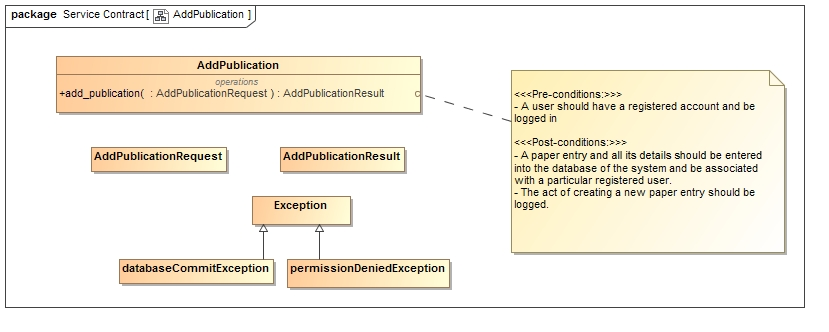
\includegraphics[width=\linewidth]{../Diagrams/ServiceContracts/Publication subsystem/AddPublication.jpg}
							\caption{Service Contract - Add Own Paper Entry}
						\end{figure}
						\begin{figure}[H]
							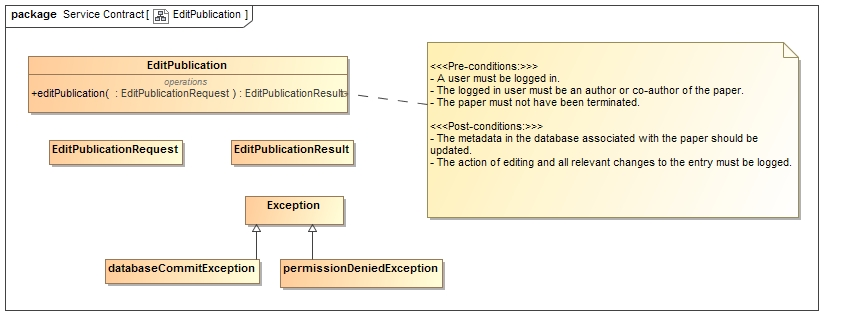
\includegraphics[width=\linewidth]{../Diagrams/ServiceContracts/Publication subsystem/EditPublication.jpg}
							\caption{Service Contract - Edit Own Paper Entry}
						\end{figure}
					\end{itemize}
					
					\item \textbf{Add/Remove Authors from a Paper:} \hfill \textit{Priority: Critical}
					\begin{itemize}
						\item A user should be able to add and remove authors from a paper which they have created or are a co-author of.
						\item \textbf{Pre-conditions:}
						\begin{itemize}
							\item The user must be logged in.
							\item The user must be the author or a co-author of the paper.
						\end{itemize}
						\item \textbf{Post-conditions:}
						\begin{itemize}
							\item There should be an ordered list of unlimited size associated with the paper consisting of the details of the author and co-authors stored in the database.
							\item The action should be logged.
						\end{itemize}
						\item \textbf{Request and Results Data Structures:}
						\begin{figure}[H]
							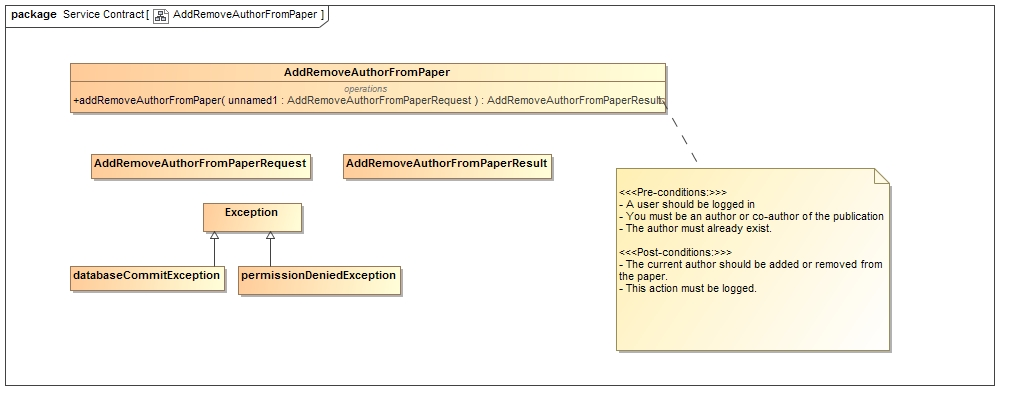
\includegraphics[width=\linewidth]{../Diagrams/ServiceContracts/Publication subsystem/AddRemoveAuthorFromPaper.jpg}
							\caption{Service Contract - Add/Remove Author from Paper}
						\end{figure}
					\end{itemize}
					
					\item \textbf{Add/Edit Author:} \hfill \textit{Priority: Critical}
					\begin{itemize}
						\item A user should have the option to add the details of a new author into the system if the author does not already exist within the system as well as edit existing authors.
						\item \textbf{Pre-conditions:}
						\begin{itemize}
							\item The user must be logged in.
							\item The author must not already exist in the case of adding.
							\item If the author does exist they should be edited.
						\end{itemize}
						\item \textbf{Post-conditions:}
						\begin{itemize}
							\item The author and his/her associated details have been added to the system's database in the case of adding.
							\item The author and his/her associated details should have been updated and stored in the database in the case of editing.
							\item The actions should be logged.
						\end{itemize}
						\item \textbf{Request and Results Data Structures:}
						\begin{figure}[H]
							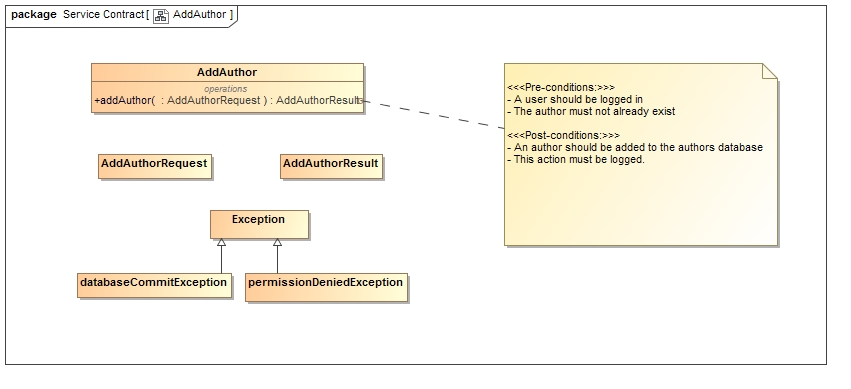
\includegraphics[width=\linewidth]{../Diagrams/ServiceContracts/Publication subsystem/AddAuthor.jpg}
							\caption{Service Contract - Add Author to System}
						\end{figure}
						\begin{figure}[H]
							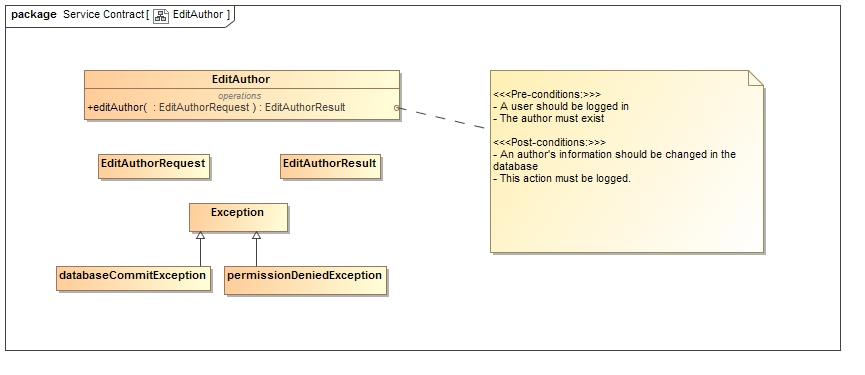
\includegraphics[width=\linewidth]{../Diagrams/ServiceContracts/Publication subsystem/EditAuthor.jpg}
							\caption{Service Contract - Edit Author}
						\end{figure}
					\end{itemize}
					
					\cleardoublepage
					\item \textbf{Edit Own Paper Progress:} \hfill \textit{Priority: Important}
					\begin{itemize}
						\item A user should have the ability to indicate using a percentage how far they are currently in terms of progress on their paper.
						\item \textbf{Pre-conditions:}
						\begin{itemize}
							\item A user should be logged in.
							\item The logged in user must be an author or co-author of the paper.
							\item The paper must not have been terminated.
						\end{itemize}
						\item \textbf{Post-conditions:}
						\begin{itemize}
							\item The field indicating progress within the database must have been updated.
							\item The change in progress should be depicted visually to the user.
							\item The action should be logged.
						\end{itemize}
						\item \textbf{Request and Results Data Structures:}
						\begin{figure}[H]
							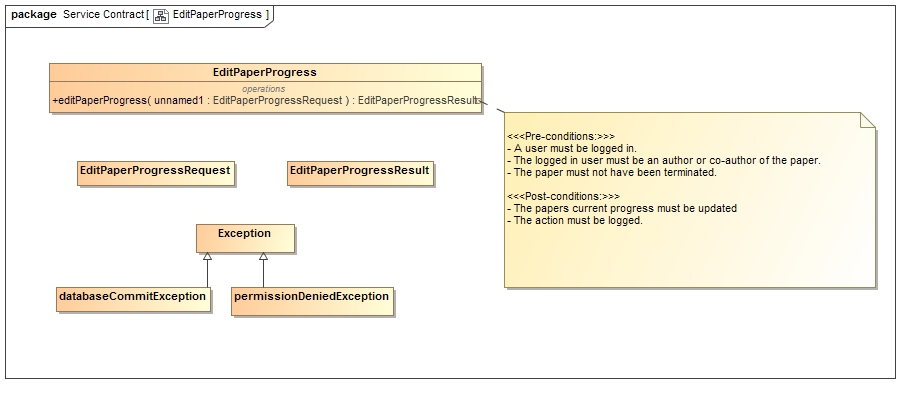
\includegraphics[width=\linewidth]{../Diagrams/ServiceContracts/Publication subsystem/EditPaperProgress.jpg}
							\caption{Service Contract - Edit Paper Progress}
						\end{figure}
					\end{itemize}			
					
					\cleardoublepage
					\item \textbf{Terminate/Resume Own Paper:} \hfill \textit{Priority: Critical}
					\begin{itemize}
						\item A user must be able to terminate (make inactive) a paper which they feel they are not going to be completing in the near future. They must also be able to resume this paper at a later stage when they want to continue work on it.
						\item \textbf{Pre-conditions:}
						\begin{itemize}
							\item A user must be logged in.
							\item The logged in user must be an author or co-author of the paper.
						\end{itemize}
						\item \textbf{Post-conditions:}
						\begin{itemize}
							\item If terminating:
							\begin{itemize}
								\item The paper has been marked as terminated within the database.
								\item The action of terminating the paper must have been logged.
								\item The paper must no longer be able to be edited by the user.
							\end{itemize}
							\item If resuming:
							\begin{itemize}
								\item The paper has been unmarked as terminated within the database.
								\item The action of resuming the paper must have been logged.
								\item The paper must be available to edit.
							\end{itemize}
						\end{itemize}
						\item \textbf{Request and Results Data Structures:}
						\begin{figure}[H]
							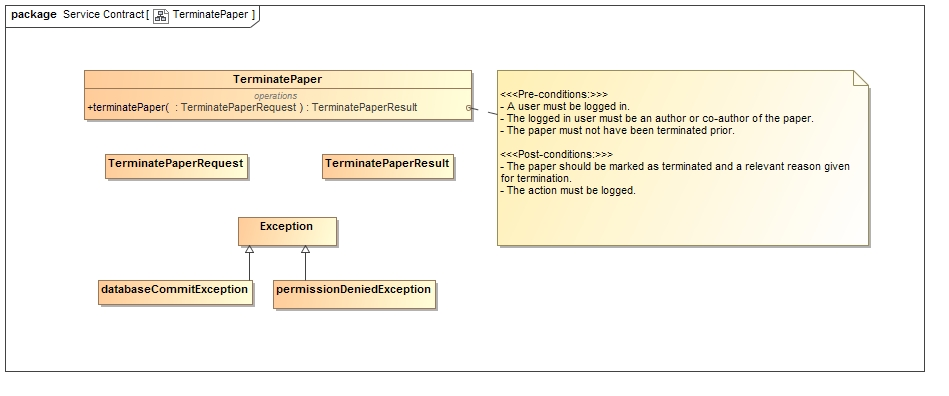
\includegraphics[width=\linewidth]{../Diagrams/ServiceContracts/Publication subsystem/TerminatePaper.jpg}
							\caption{Service Contract - Terminate Paper}
						\end{figure}
						\begin{figure}[H]
							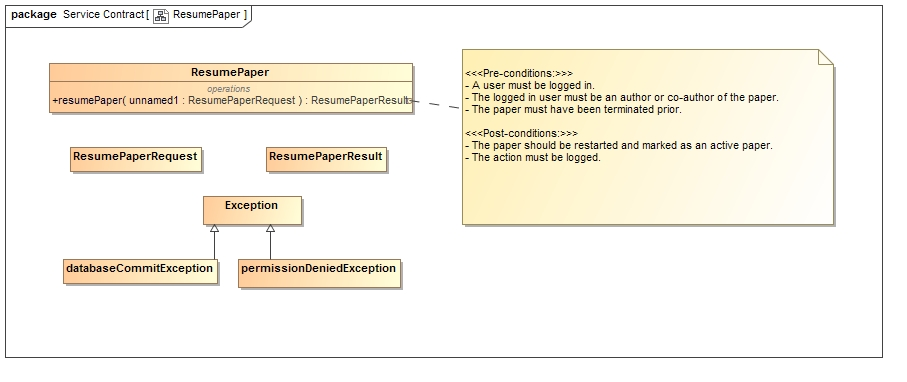
\includegraphics[width=\linewidth]{../Diagrams/ServiceContracts/Publication subsystem/ResumePaper.jpg}
							\caption{Service Contract - Resume Paper}
						\end{figure}
					\end{itemize}
					
					\cleardoublepage
					\item \textbf{Add/Remove Conference/Journal to Paper:} \hfill \textit{Priority: Critical}
					\begin{itemize}
						\item Whilst creating or editing a paper a user should be able to associate a particular conference or journal with their paper as well as be able to remove an already associated conference or journal whilst editing a paper.
						\item \textbf{Pre-conditions:}
						\begin{itemize}
							\item The user must be logged in.
							\item The user must be an author or co-author of the paper in question.
						\end{itemize}
						\item \textbf{Post-conditions:}
						\begin{itemize}
							\item The paper should be associated with a particular conference or journal or the paper should have had its association removed.
							\item The action should be logged.
						\end{itemize}
						\item \textbf{Request and Results Data Structures:}
						\begin{figure}[H]
							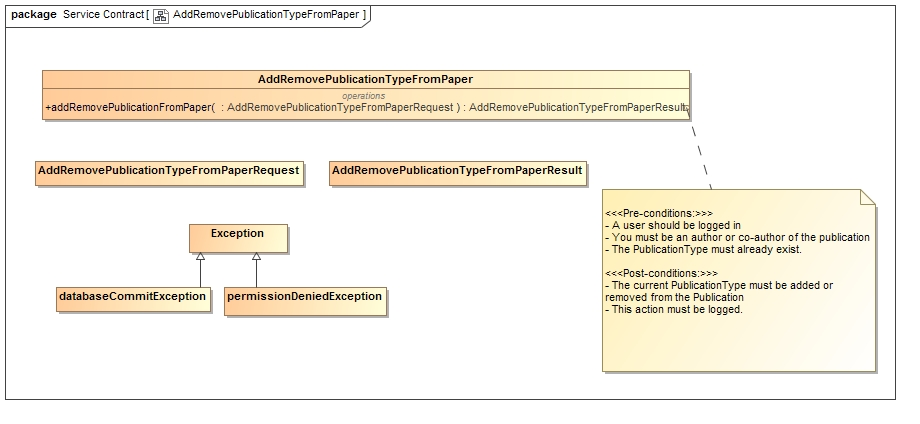
\includegraphics[width=\linewidth]{../Diagrams/ServiceContracts/Publication subsystem/AddRemovePublicationTypeFromPaper.jpg}
							\caption{Service Contract - Add/Remove Publication Type from Paper}
						\end{figure}
					\end{itemize}									
					
					\cleardoublepage
					\item \textbf{Add/Edit Conference/Journal:} \hfill \textit{Priority: Critical}
					\begin{itemize}
						\item A user must be able to fill in the details of a particular conference or journal if it does not already exist within the system. If it does exist the user should be able to edit it.
						\item \textbf{Pre-conditions:}
						\begin{itemize}
							\item The user must be logged in.
							\item The conference or journal must not already exist.
						\end{itemize}
						\item \textbf{Post-conditions:}
						\begin{itemize}
							\item The conference or journal and all its details have been added to the system's database in the case of adding.
							\item In the case of editing the conference/journal must have been updated within the database.
							\item The actions have been logged.
						\end{itemize}
						\item \textbf{Request and Results Data Structures:}
						\begin{figure}[H]
							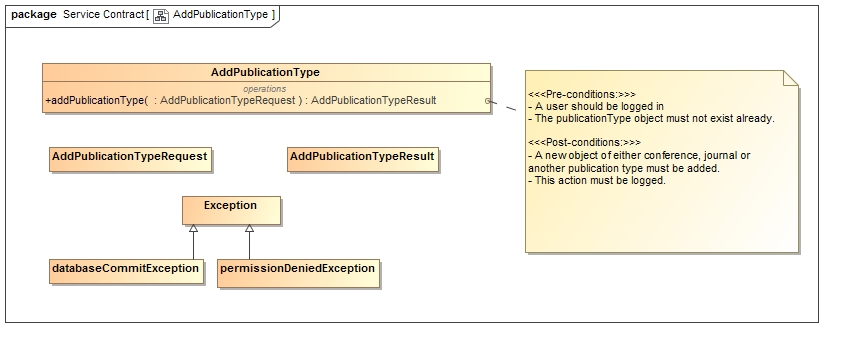
\includegraphics[width=\linewidth]{../Diagrams/ServiceContracts/Publication subsystem/AddPublicationType.jpg}
							\caption{Service Contract - Add Publication Type}
						\end{figure}
						\begin{figure}[H]
							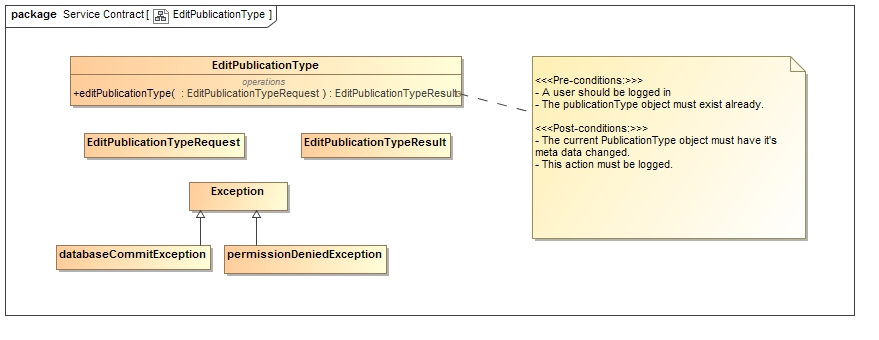
\includegraphics[width=\linewidth]{../Diagrams/ServiceContracts/Publication subsystem/EditPublicationType.jpg}
							\caption{Service Contract - Edit Publication Type}
						\end{figure}
					\end{itemize}								
				\end{itemize}
				\cleardoublepage
				\textbf{Head of Research:}
				
				\begin{itemize}
					\item \textbf{Search All Papers Within Own Research Group} \hfill \textit{Priority: Critical}
					\begin{itemize}
						\item The head of a research group should have access to all the papers associated with their particular research group.
						\item \textbf{Pre-conditions:}
						\begin{itemize}
							\item The user must be logged in.
							\item The user must be the head of the particular research group they would like to observe.
						\end{itemize}
						\item \textbf{Post-conditions:}
						\begin{itemize}
							\item The user should be able to view all metadata associated with the papers of their research group.
							\item The action should be logged.
						\end{itemize}
						\item \textbf{Request and Results Data Structures:}
						\begin{figure}[H]
							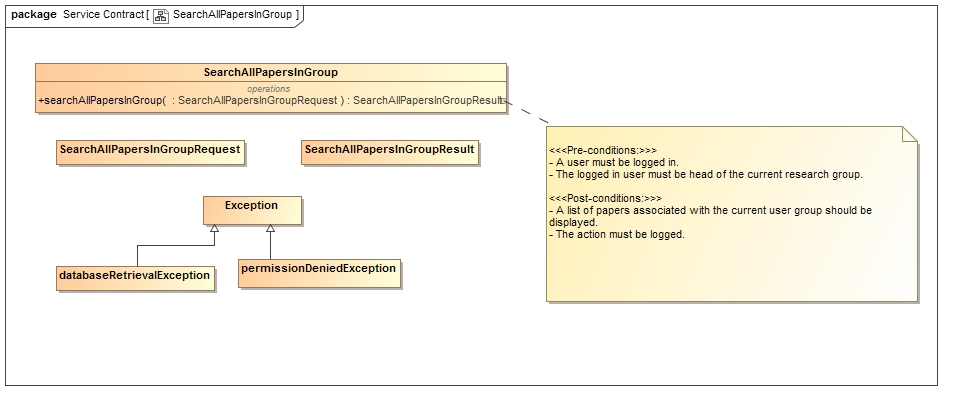
\includegraphics[width=\linewidth]{../Diagrams/ServiceContracts/Publication subsystem/SearchAllPapersInGroup.jpg}
							\caption{Service Contract - Search All Papers in Group}
						\end{figure}
					\end{itemize}
				\end{itemize}
				
				\cleardoublepage
				\textbf{Admin:}
				
				\begin{itemize}
					\item \textbf{Search All Papers on System} \hfill \textit{Priority: Critical}
					\begin{itemize}
						\item An admin user should be able to view all papers and their metadata on the system.
						\item \textbf{Pre-conditions:}
						\begin{itemize}
							\item The user must be logged in.
							\item The user must have the privilege rights assigned to an admin.
						\end{itemize}
						\item \textbf{Post-conditions:}
						\begin{itemize}
							\item The user should be able to view all metadata associated with all the papers stored on the system.
							\item The action should be logged.
						\end{itemize}
						\item \textbf{Request and Results Data Structures:}
						\begin{figure}[H]
							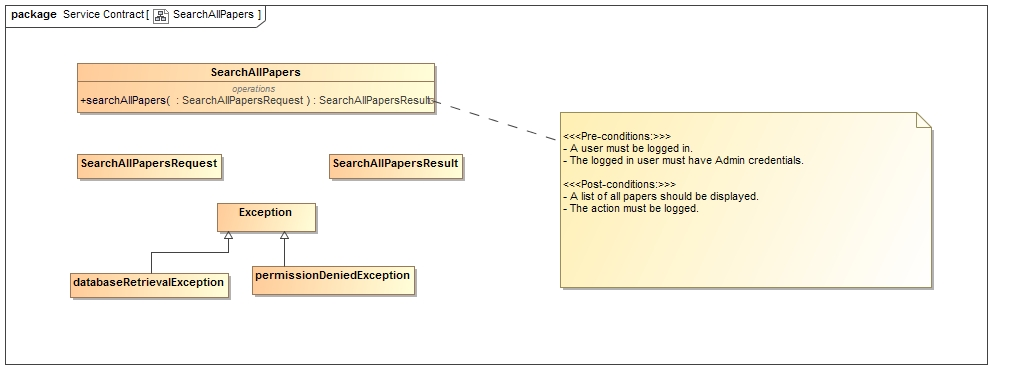
\includegraphics[width=\linewidth]{../Diagrams/ServiceContracts/Publication subsystem/SearchAllPapers.jpg}
							\caption{Service Contract - Search All Papers}
						\end{figure}
					\end{itemize}
					
					\cleardoublepage
					\item \textbf{Purge Paper From the System} \hfill \textit{Priority: Important}
					\begin{itemize}
						\item An admin user should be able to completely remove a paper from the system if they find the need to do so.
						\item \textbf{Pre-conditions:}
						\begin{itemize}
							\item The user must be logged in.
							\item The user must have the privilege rights assigned to an admin.
						\end{itemize}
						\item \textbf{Post-conditions:}
						\begin{itemize}
							\item The paper and all of its metadata should be permanently removed from the system.
							\item The action should be logged.
						\end{itemize}
						\item \textbf{Request and Results Data Structures:}
						\begin{figure}[H]
							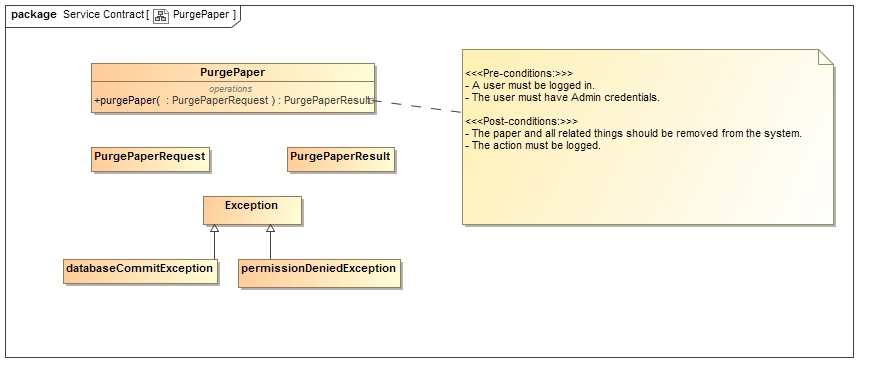
\includegraphics[width=\linewidth]{../Diagrams/ServiceContracts/Publication subsystem/PurgePaper.jpg}
							\caption{Service Contract - Purge Paper}
						\end{figure}
					\end{itemize}
				\end{itemize}
			\cleardoublepage
			\subsubsection{User Sub-System}\label{subsubsec:user}
				Handles all actions associated with user accounts such as login, viewing and editing profiles, as well as privileged actions such as adding/removing users to the system and adding/removing users from a research group.\\
				[3mm]
				\textbf{User:}
				\begin{itemize}
					\item \textbf{Login} \hfill \textit{Priority: Critical}
					\begin{itemize}
						\item A registered user of the system must be able to login to the system using their private credentials.
						\item \textbf{Pre-conditions:}
						\begin{itemize}
							\item The user must not be logged in.
							\item The identifying field used (email address) must match one of an active, registered user of the system.
							\item The password entered must match the password associated with the identifying field within the system.
						\end{itemize}
						\item \textbf{Post-conditions:}
						\begin{itemize}
							\item The system must begin a session for the user.
							\item The user must gain access to the system according to the set of privileges associated with their account.		
							\item The action should be logged.
						\end{itemize}
						\item \textbf{Request and Results Data Structures:}
						\begin{figure}[H]
							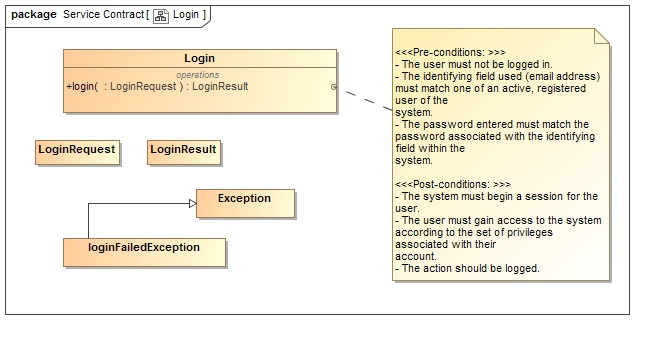
\includegraphics[width=\linewidth]{../Diagrams/ServiceContracts/User subsystem/Login.jpg}
							\caption{Service Contract - Login}
						\end{figure}
					\end{itemize}
					
					\cleardoublepage
					\item \textbf{Logout} \hfill \textit{Priority: Critical}
					\begin{itemize}
						\item A user must be able to end their session and log out of the system.
						\item \textbf{Pre-conditions:}
						\begin{itemize}
							\item A user must be logged in.
						\end{itemize}
						\item \textbf{Post-conditions:}
						\begin{itemize}
							\item The user's session must be ended and the user must no longer be logged in.
						\end{itemize}
						\item \textbf{Request and Results Data Structures:}
						\begin{figure}[H]
							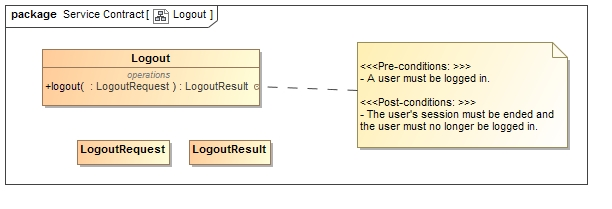
\includegraphics[width=\linewidth]{../Diagrams/ServiceContracts/User subsystem/Logout.jpg}
							\caption{Service Contract - Logout}
						\end{figure}
					\end{itemize}
					
					\cleardoublepage
					\item \textbf{View Own User Profile} \hfill \textit{Priority: Critical}
					\begin{itemize}
						\item A logged in user should be able to see their own profile and all details associated with it. The user should also be able to view all papers associated with their account.
						\item \textbf{Pre-conditions:}
						\begin{itemize}
							\item The user must be logged in.
							\item The user's profile being viewed must be the same as the logged in user.
						\end{itemize}
						\item \textbf{Post-conditions:}
						\begin{itemize}
							\item The information associated with the user's account should be displayed to them.
							\item The action should be logged.
						\end{itemize}
						\item \textbf{Request and Results Data Structures:}
						\begin{figure}[H]
							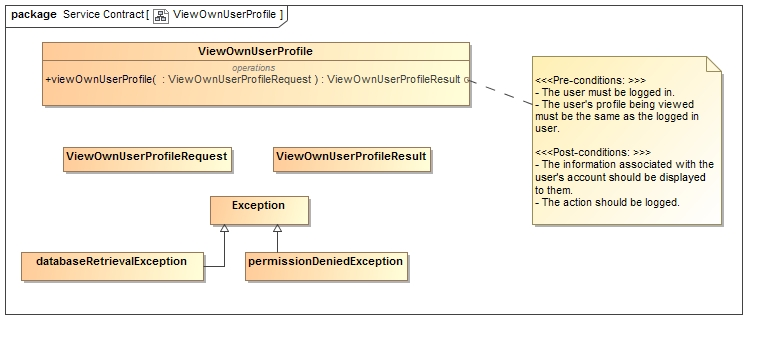
\includegraphics[width=\linewidth]{../Diagrams/ServiceContracts/User subsystem/ViewOwnUserProfile.jpg}
							\caption{Service Contract - View Own User Profile}
						\end{figure}
					\end{itemize}
					
					\cleardoublepage
					\item \textbf{Edit Own User Profile} \hfill \textit{Priority: Critical}
					\begin{itemize}
						\item A logged in user should be able to edit all details associated with their user account.
						\item \textbf{Pre-conditions:}
						\begin{itemize}
							\item The user must be logged in.
							\item The user profile being edited must belong to the user editing it.
						\end{itemize}
						\item \textbf{Post-conditions:}
						\begin{itemize}
							\item The updated information associated with the user's account should be stored in the system.
							\item The action should be logged.
						\end{itemize}
						\item \textbf{Request and Results Data Structures:}
						\begin{figure}[H]
							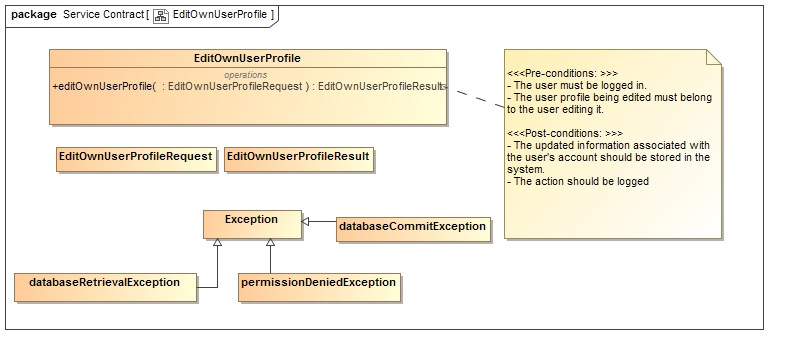
\includegraphics[width=\linewidth]{../Diagrams/ServiceContracts/User subsystem/EditOwnUserProfile.jpg}
							\caption{Service Contract - Edit Own User Profile}
						\end{figure}
					\end{itemize}							
				\end{itemize}
				\cleardoublepage
				\textbf{Head of Research:}
				
				\begin{itemize}
					\item \textbf{Add/Remove Users from Own Research Group} \hfill \textit{Priority: Critical}
					\begin{itemize}
						\item The head of a research group should be able to manage the users associated with that group.
						\item \textbf{Pre-conditions:}
						\begin{itemize}
							\item The user must be logged in.
							\item The user must have the privileges associated with a Head of Research.
							\item The user must be the Head of Research of the particular group which they are wanting to manage.
						\end{itemize}
						\item \textbf{Post-conditions:}
						\begin{itemize}
							\item The user must have been able to add other registered users into their research group.
							\item The user must have been able to remove other registered users from their research group.
							\item The action should be logged.
						\end{itemize}
						\item \textbf{Request and Results Data Structures:}
						\begin{figure}[H]
							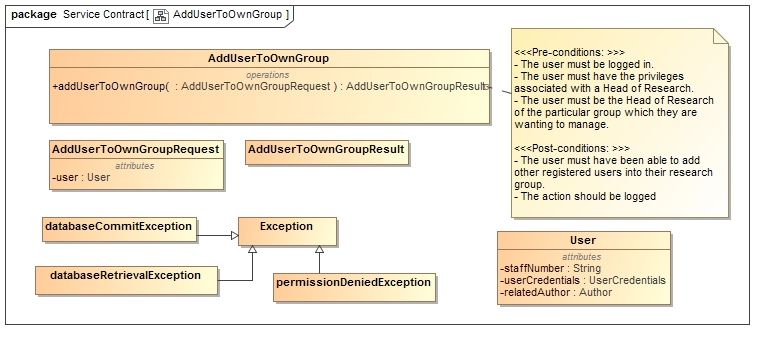
\includegraphics[width=\linewidth]{../Diagrams/ServiceContracts/User subsystem/AddUserToOwnGroup.jpg}
							\caption{Service Contract - Add User to Own Group}
						\end{figure}
						\begin{figure}[H]
							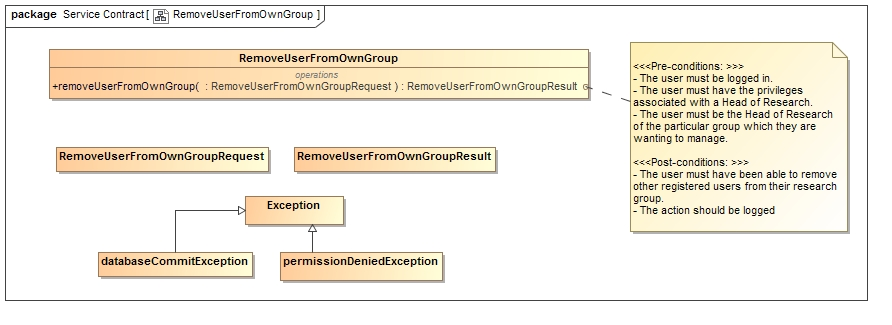
\includegraphics[width=\linewidth]{../Diagrams/ServiceContracts/User subsystem/RemoveUserFromOwnGroup.jpg}
							\caption{Service Contract - Remove User from Own Group}
						\end{figure}
					\end{itemize}
					
					\cleardoublepage
					\item \textbf{Search/View All Users in Own Research Group} \hfill \textit{Priority: Critical}
					\begin{itemize}
						\item The head of a research group should be able to search all of the users within their research group. They should also be able to access the profiles and information associated with the users within their research group. In particular the head of a research group should be able to view all paper entries associated with each user.
						\item \textbf{Pre-conditions:}
						\begin{itemize}
							\item The user must be logged in.
							\item The user must be the Head of Research of the particular group which they are wanting to search/view.
						\end{itemize}
						\item \textbf{Post-conditions:}
						\begin{itemize}
							\item The user must have been able to view all of the users associated with their research group.
							\item The head of the research group can access and view all profile information (including paper entries) for each of the users associated with their research group.
							\item The action should be logged.
						\end{itemize}
						\item \textbf{Request and Results Data Structures:}
						\begin{figure}[H]
							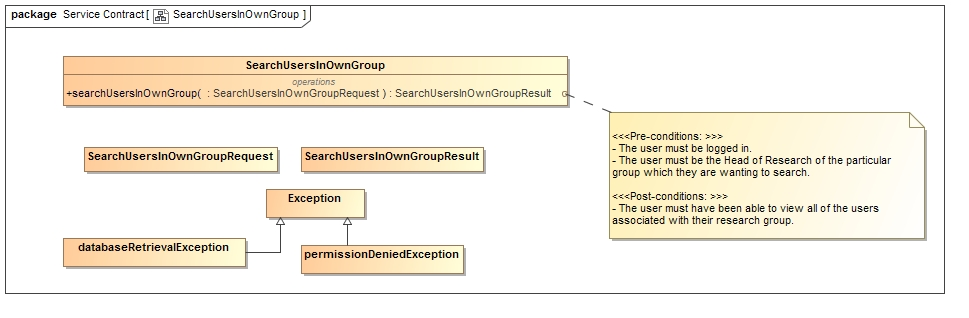
\includegraphics[width=\linewidth]{../Diagrams/ServiceContracts/User subsystem/SearchUsersInOwnGroup.jpg}
							\caption{Service Contract - Search Users in Own Group}
						\end{figure}
						\begin{figure}[H]
							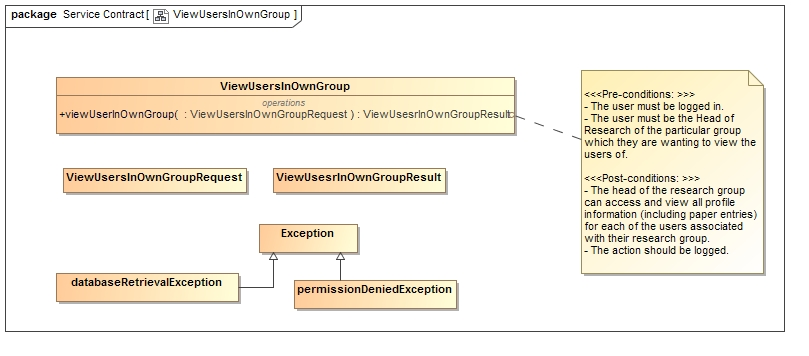
\includegraphics[width=\linewidth]{../Diagrams/ServiceContracts/User subsystem/ViewUsersInOwnGroup.jpg}
							\caption{Service Contract - View User in Own Group}
						\end{figure}
					\end{itemize}
				\end{itemize}
				
				\cleardoublepage
				\textbf{Admin:}
				
				\begin{itemize}
					\item \textbf{Add New User to System} \hfill \textit{Priority: Critical}
					\begin{itemize}
						\item Admin users should have the ability to add new users into the system.
						\item \textbf{Pre-conditions:}
						\begin{itemize}
							\item The user must be logged in.
							\item The user must have the privileges associated with an admin account.
						\end{itemize}
						\item \textbf{Post-conditions:}
						\begin{itemize}
							\item A new user with all their metadata as well as privileges should be added into the system.
							\item The action should be logged.
						\end{itemize}
						\item \textbf{Request and Results Data Structures:}
						\begin{figure}[H]
							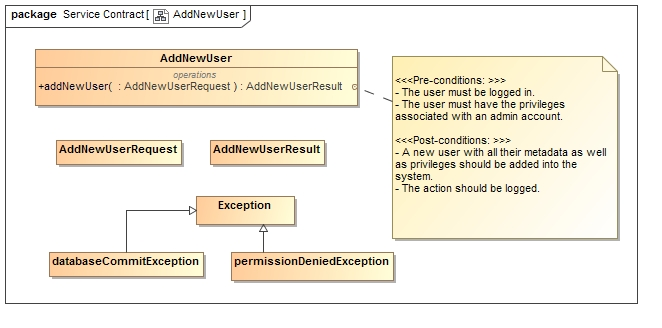
\includegraphics[width=\linewidth]{../Diagrams/ServiceContracts/User subsystem/AddNewUser.jpg}
							\caption{Service Contract - Add New User}
						\end{figure}
					\end{itemize}
					
					\cleardoublepage
					\item \textbf{Search/View All Users in Any Research Group} \hfill \textit{Priority: Critical}
					\begin{itemize}
						\item Admin users should be able to search through all of the users within the system as well as view their profiles and all associated data and papers.
						\item \textbf{Pre-conditions:}
						\begin{itemize}
							\item The user must be logged in.
							\item The user must have the privileges associated with an admin account.
						\end{itemize}
						\item \textbf{Post-conditions:}
						\begin{itemize}
							\item The admin user should have been able to search and locate particular registered users on the system.
							\item All information, paper entries and their metadata should be available for viewing to the admin user. Upon selecting a particular user all information associated with that user is displayed.
							\item This action should be logged.
						\end{itemize}
						\item \textbf{Request and Results Data Structures:}
						\begin{figure}[H]
							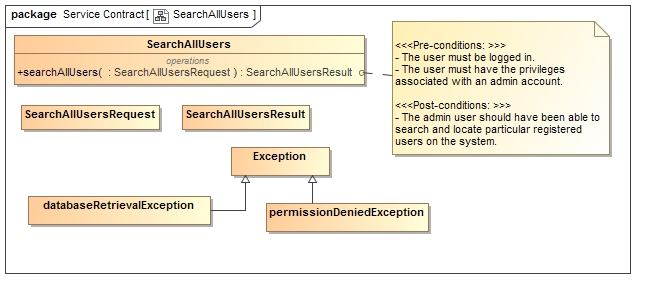
\includegraphics[width=\linewidth]{../Diagrams/ServiceContracts/User subsystem/SearchAllUsers.jpg}
							\caption{Service Contract - Search All Users}
						\end{figure}
						\begin{figure}[H]
							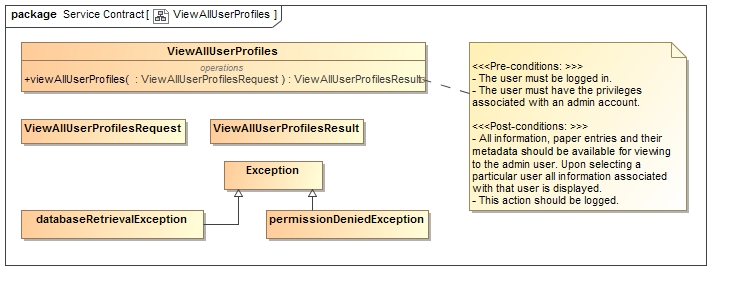
\includegraphics[width=\linewidth]{../Diagrams/ServiceContracts/User subsystem/ViewAllUserProfiles.jpg}
							\caption{Service Contract - View All User Profiles}
						\end{figure}
					\end{itemize}
					
					\cleardoublepage
					\item \textbf{Purge User from System} \hfill \textit{Priority: Important}
					\begin{itemize}
						\item An admin user must be able to permanently remove a user and all of their associated information from the system.
						\item \textbf{Pre-conditions:}
						\begin{itemize}
							\item The user must be logged in.
							\item The user must have the privileges associated with an admin account.
							\item The user must confirm they want to continue with the action before the system executes the command.
						\end{itemize}
						\item \textbf{Post-conditions:}
						\begin{itemize}
							\item The user and all of their associated information should be removed from the system.
							\item The action should be logged.
						\end{itemize}
						\item \textbf{Request and Results Data Structures:}
						\begin{figure}[H]
							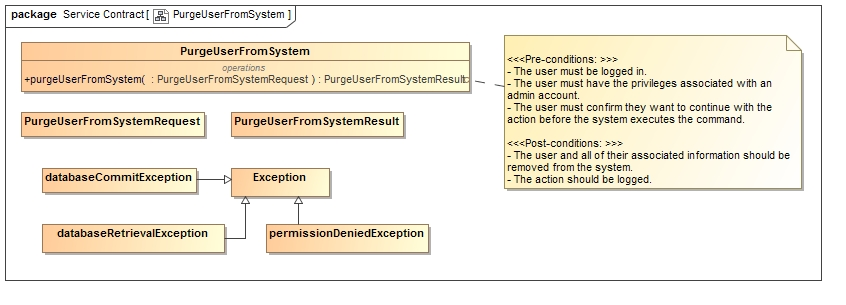
\includegraphics[width=\linewidth]{../Diagrams/ServiceContracts/User subsystem/PurgeUserFromSystem.jpg}
							\caption{Service Contract - Purge User From System}
						\end{figure}
					\end{itemize}
					
					\cleardoublepage
					\item \textbf{Set User as Active/Inactive} \hfill \textit{Priority: Important}
					\begin{itemize}
						\item An admin user should be able to set the status of a user to active or inactive, allowing the user to login or preventing them from continuing to interact with the system.
						\item \textbf{Pre-conditions:}
						\begin{itemize}
							\item The user must be logged in.
							\item The user must have the privileges associated with an admin account.
						\end{itemize}
						\item \textbf{Post-conditions:}
						\begin{itemize}
							\item The selected user should have been marked as active/inactive, active allowing the user to login and use the system, inactive preventing them from login in to the system and making changes.
							\item The action should be logged.
						\end{itemize}
						\item \textbf{Request and Results Data Structures:}
						\begin{figure}[H]
							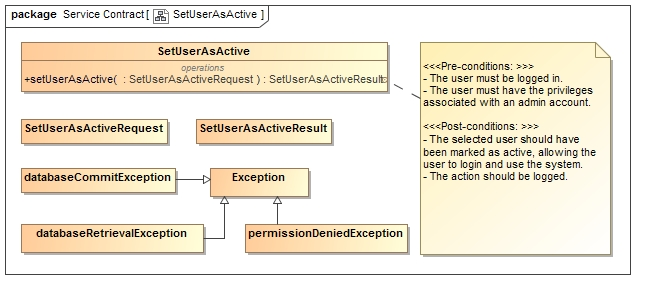
\includegraphics[width=\linewidth]{../Diagrams/ServiceContracts/User subsystem/SetUserAsActive.jpg}
							\caption{Service Contract - Set User as Active}
						\end{figure}
						\begin{figure}[H]
							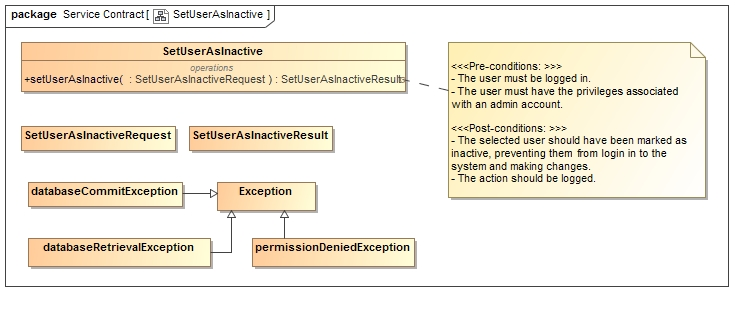
\includegraphics[width=\linewidth]{../Diagrams/ServiceContracts/User subsystem/SetUserAsInactive.jpg}
							\caption{Service Contract - Set User as Inactive}
						\end{figure}
					\end{itemize}
					
					\cleardoublepage
					\item \textbf{Add/Remove Users From Any Research Group} \hfill \textit{Priority: Critical}
					\begin{itemize}
						\item An admin user should be able to add or remove a user from any of the research groups within the system.
						\item \textbf{Pre-conditions:}
						\begin{itemize}
							\item The user must be logged in.
							\item The user must have the privileges associated with an admin account.
						\end{itemize}
						\item \textbf{Post-conditions:}
						\begin{itemize}
							\item The selected user should be associated with the specified research group in the case of adding and should be removed and no longer associated with a research group in the case of removing.
							\item The action should be logged.
						\end{itemize}
						\item \textbf{Request and Results Data Structures:}
						\begin{figure}[H]
							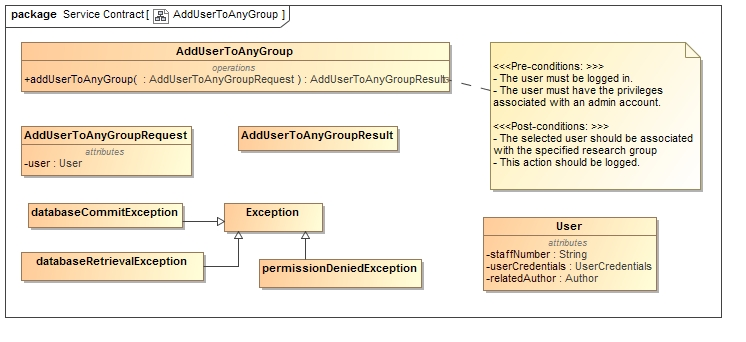
\includegraphics[width=\linewidth]{../Diagrams/ServiceContracts/User subsystem/AddUserToAnyGroup.jpg}
							\caption{Service Contract - Add User to Any Group}
						\end{figure}
						\begin{figure}[H]
							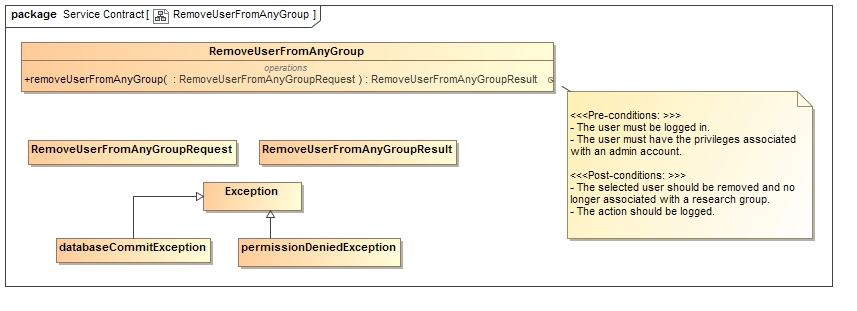
\includegraphics[width=\linewidth]{../Diagrams/ServiceContracts/User subsystem/RemoveUserFromAnyGroup.jpg}
							\caption{Service Contract - Remove User from Any Group}
						\end{figure}
					\end{itemize}
				\end{itemize}
				
				\cleardoublepage
			\subsubsection{Notification Sub-System}\label{subsubsec:notification}
				Handles the adding and editing of notifications within the system, as well the process of creating and sending notifications to relevant users of the system.\\
				[3mm]
				\textbf{User:}
				\begin{itemize}
					\item \textbf{Update Paper Deadline} \hfill \textit{Priority: Important}
					\begin{itemize}
						\item Upon creating a paper entry a user must be able to set/update the deadline for when the paper needs to be published by.
						\item \textbf{Pre-conditions:}
						\begin{itemize}
							\item The user must be logged in.
							\item The user must be the author or a co-author of the paper which they would like to set the deadline for.
							\item The paper must not have been terminated.
						\end{itemize}
						\item \textbf{Post-conditions:}
						\begin{itemize}
							\item A deadline will have been set and stored in the system. It will be associated with the particular paper on which it was set.
							\item An update notification should be sent to authors of the paper indicating that the deadline has been set.
							\item The action should be logged.
						\end{itemize}
						\item \textbf{Request and Results Data Structures:}
						\begin{figure}[H]
							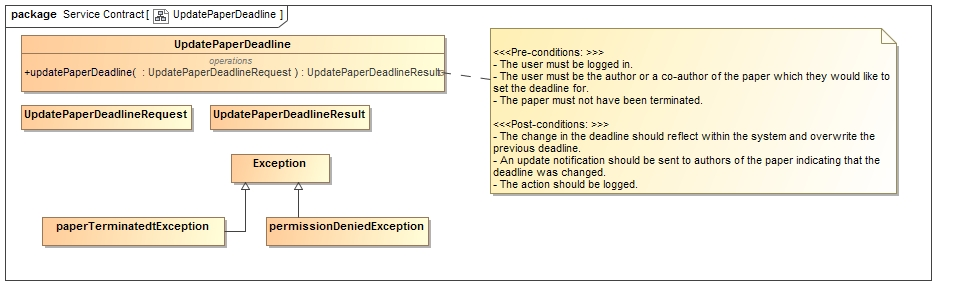
\includegraphics[width=\linewidth]{../Diagrams/ServiceContracts/Notification subsystem/UpdatePaperDeadline.jpg}
							\caption{Service Contract - Update Paper Deadline}
						\end{figure}
					\end{itemize}						
				\end{itemize}
				
				\cleardoublepage
				\textbf{\large{Date and Time:}}
				\begin{itemize}
					\item \textbf{Send Deadline Notification} \hfill \textit{Priority: Important}
					\begin{itemize}
						\item The system must be able to notify an author as well as co-authors of a paper of the deadline for the paper.
						\item \textbf{Pre-conditions:}
						\begin{itemize}
							\item A deadline must have been set for a paper.
							\item The deadline must not have passed already.
							\item The authors being notified must be associated with the paper the deadline has been set on.
						\end{itemize}
						\item \textbf{Post-conditions:}
						\begin{itemize}
							\item Authors of a particular paper are notified via the use of email as to what the deadline for the paper is.
							\item The action should be logged.
						\end{itemize}
						\item \textbf{Request and Results Data Structures:}
						\begin{figure}[H]
							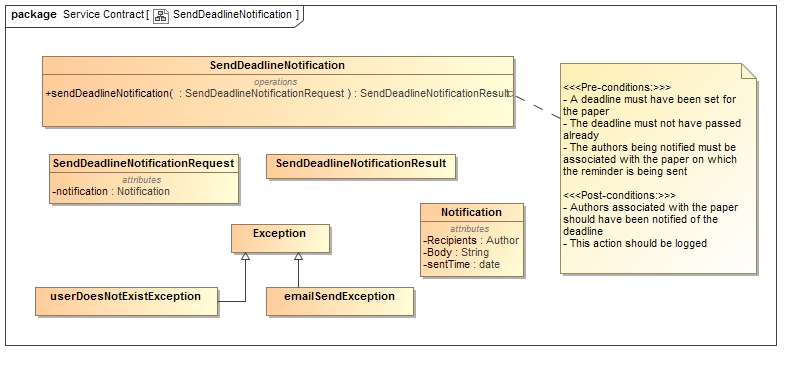
\includegraphics[width=\linewidth]{../Diagrams/ServiceContracts/Notification subsystem/SendDeadlineNotification.jpg}
							\caption{Service Contract - Send Deadline Notification}
						\end{figure}
					\end{itemize}
					
					\item \textbf{Send Deadline Update Notification} \hfill \textit{Priority: Important}
					\begin{itemize}
						\item The system must be able to notify an author as well as co-authors of a paper when the deadline for a paper is updated.
						\item \textbf{Pre-conditions:}
						\begin{itemize}
							\item The user must be logged in.
							\item A new deadline must have been set for a paper.
							\item The deadline must not have passed already.
							\item The authors being notified must be associated with the paper the deadline has been updated on.
						\end{itemize}
						\item \textbf{Post-conditions:}
						\begin{itemize}
							\item Authors of a particular paper are notified via the use of email as to what the updated deadline for the paper is.
							\item The action should be logged.
						\end{itemize}
						\item \textbf{Request and Results Data Structures:}
						\begin{figure}[H]
							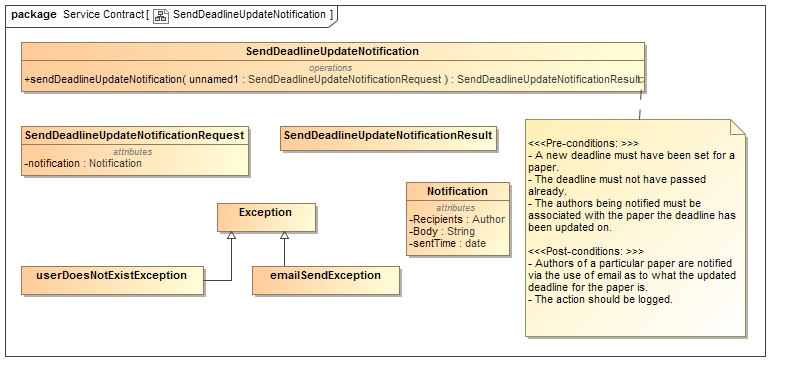
\includegraphics[width=\linewidth]{../Diagrams/ServiceContracts/Notification subsystem/SendDeadlineUpdateNotification.jpg}
							\caption{Service Contract - Send Deadline Update Notification}
						\end{figure}
					\end{itemize}
				\end{itemize}
				
			\cleardoublepage
			\subsubsection{Reporting Sub-System}\label{subsubsec:report}
				Handles the generation of reports with regards to all relevant information contained by the system.\\
				[3mm]
				\textbf{Head of Research:}
				\begin{itemize}
					\item \textbf{Generate Report for Research Group} \hfill \textit{Priority: Important}
					\begin{itemize}
						\item The head of a research group should be able to generate a summarised report of all important information related to their research group in terms of the users in the group as well as their papers and all metadata associated with their papers.
						\item \textbf{Pre-conditions:}
						\begin{itemize}
							\item The user must be logged in.
							\item The user must have the privileges associated with a Head of Research.
							\item The user must be the head of the research group which they would like to generate a report on.
						\end{itemize}
						\item \textbf{Post-conditions:}
						\begin{itemize}
							\item The head of the research group should have all relevant information returned to him/her in a summarised and easily readable manner.
							\item This action should be logged.
						\end{itemize}
						\item \textbf{Request and Results Data Structures:}
						\begin{figure}[H]
							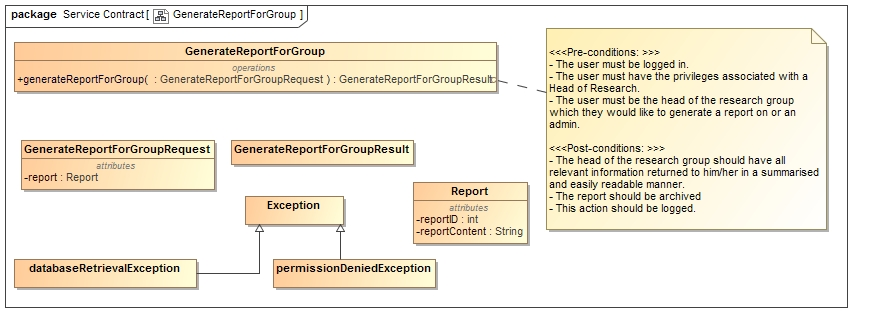
\includegraphics[width=\linewidth]{../Diagrams/ServiceContracts/Reporting subsystem/GenerateReportForGroup.jpg}
							\caption{Service Contract - Generate Report for Group}
						\end{figure}
					\end{itemize}
				\end{itemize}
				
				\cleardoublepage
				\textbf{Admin:}
				\begin{itemize}
					\item \textbf{Generate Report for Department} \hfill \textit{Priority: Important}
					\begin{itemize}
						\item An admin user should be able to generate a summarised report of all important information related to their department as a whole. This includes summaries of each research group and associated papers, as well as of each individual user of the system and their associated papers.
						\item \textbf{Pre-conditions:}
						\begin{itemize}
							\item The user must be logged in.
							\item The user must have the privileges associated with an admin.
						\end{itemize}
						\item \textbf{Post-conditions:}
						\begin{itemize}
							\item The admin should have all relevant information returned to him/her in a summarised and easily readable manner.
							\item The action should be logged.
						\end{itemize}
						\item \textbf{Request and Results Data Structures:}
						\begin{figure}[H]
							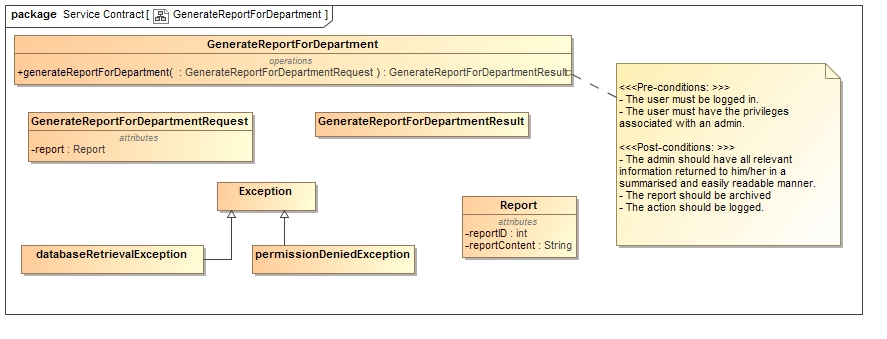
\includegraphics[width=\linewidth]{../Diagrams/ServiceContracts/Reporting subsystem/GenerateReportForDepartment.jpg}
							\caption{Service Contract - Generate Report for Department}
						\end{figure}
					\end{itemize}

					\cleardoublepage
					\item \textbf{Dump Database to File} \hfill \textit{Priority: Nice-to-Have}
					\begin{itemize}
						\item An admin user should be able to at any point dump all of the information within the database into a file for safekeeping, such as a CSV file.
						\item \textbf{Pre-conditions:}
						\begin{itemize}
							\item The user must be logged in.
							\item The user must have the privileges associated with an admin user.
						\end{itemize}
						\item \textbf{Post-conditions:}
						\begin{itemize}
							\item All information contained in the database should be dumped into a CSV file and be made available to download by the admin user.
							\item This action should be logged.
						\end{itemize}
						\item \textbf{Request and Results Data Structures:}
						\begin{figure}[H]
							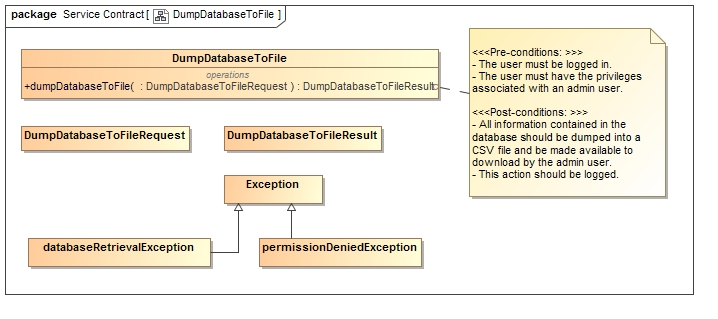
\includegraphics[width=\linewidth]{../Diagrams/ServiceContracts/Reporting subsystem/DumpDatabaseToFile.jpg}
							\caption{Service Contract - Dump Database to File}
						\end{figure}
					\end{itemize}
				\end{itemize}
			
			\cleardoublepage
			\subsubsection{Group-Control Sub-System}\label{subsubsec:group}
				Handles the creating and removing of research groups, as well as the allocating of heads of research groups and the editing of individual research groups associated metadata.\\
				[3mm]
				\textbf{Head of Research:}
				\begin{itemize}
					\item \textbf{Edit Research Group Information} \hfill \textit{Priority: Critical}
					\begin{itemize}
						\item A head of a research group should be able to edit the information associated with their research group.
						\item \textbf{Pre-conditions:}
						\begin{itemize}
							\item The user must be logged in.
							\item The user must have the privileges associated with a research leader.
							\item The user must be the head of the research group which they are attempting to edit the information of.
						\end{itemize}
						\item \textbf{Post-conditions:}
						\begin{itemize}
							\item The information associated with the particular research group should have been updated within the system.
							\item This action should be logged.
						\end{itemize}
						\item \textbf{Request and Results Data Structures:}
						\begin{figure}[H]
							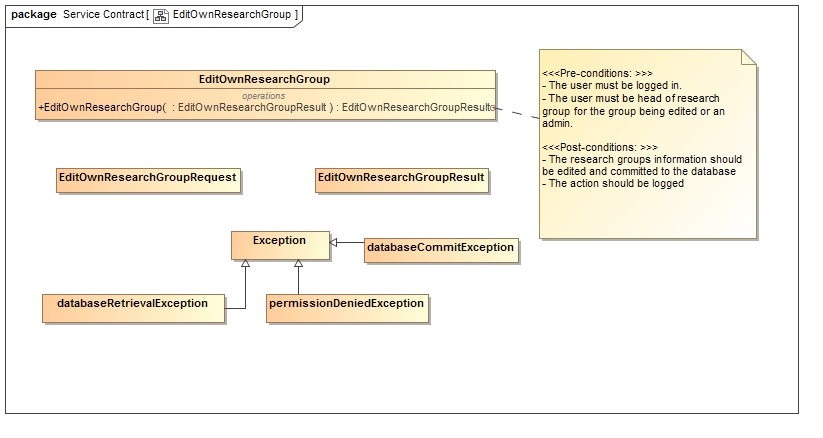
\includegraphics[width=\linewidth]{../Diagrams/ServiceContracts/Group control subsystem/EditOwnResearchGroup.jpg}
							\caption{Service Contract - Edit Own Research Group}
						\end{figure}
					\end{itemize}
				\end{itemize}
				
				\cleardoublepage
				\textbf{Admin:}
				\begin{itemize}
					\item \textbf{Add Research Group} \hfill \textit{Priority: Critical}
					\begin{itemize}
						\item An admin user should be able to add research groups to the system.
						\item \textbf{Pre-conditions:}
						\begin{itemize}
							\item The user must be logged in.
							\item The user must have the privileges associated with an admin user.
						\end{itemize}
						\item \textbf{Post-conditions:}
						\begin{itemize}
							\item A new research group which is able to have users added to or removed from should exist within the system.
							\item The action should be logged.
						\end{itemize}
						\item \textbf{Request and Results Data Structures:}
						\begin{figure}[H]
							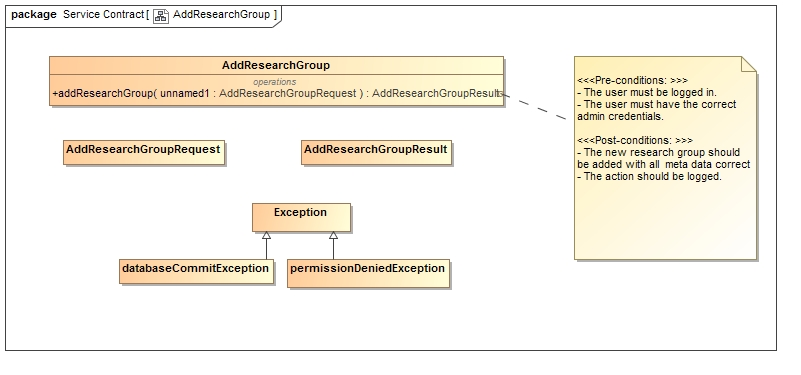
\includegraphics[width=\linewidth]{../Diagrams/ServiceContracts/Group control subsystem/AddResearchGroup.jpg}
							\caption{Service Contract - Add Research Group}
						\end{figure}
					\end{itemize}
					
					\cleardoublepage
					\item \textbf{Set Research Group as Active/Inactive} \hfill \textit{Priority: Important}
					\begin{itemize}
						\item An admin user should be able to set a research group as being active or inactive.
						\item \textbf{Pre-conditions:}
						\begin{itemize}
							\item The user must be logged in.
							\item The user must have the privileges associated with an admin user.
						\end{itemize}
						\item \textbf{Post-conditions:}
						\begin{itemize}
							\item In the case of setting active the research group should be able to have its information edited and have users added to and removed from the group.
							\item In the case of setting inactive the research group should no longer be able to have any operations performed on it.
							\item In both cases the action should be logged.
						\end{itemize}
						\item \textbf{Request and Results Data Structures:}
						\begin{figure}[H]
							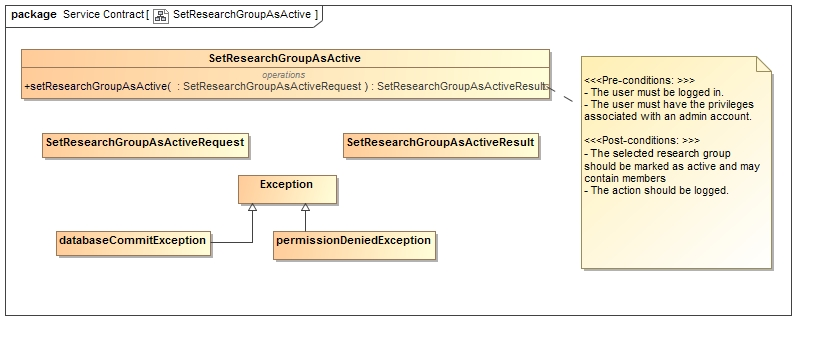
\includegraphics[width=\linewidth]{../Diagrams/ServiceContracts/Group control subsystem/SetResearchGroupAsActive.jpg}
							\caption{Service Contract - Set Research Group as Active}
						\end{figure}
						\begin{figure}[H]
							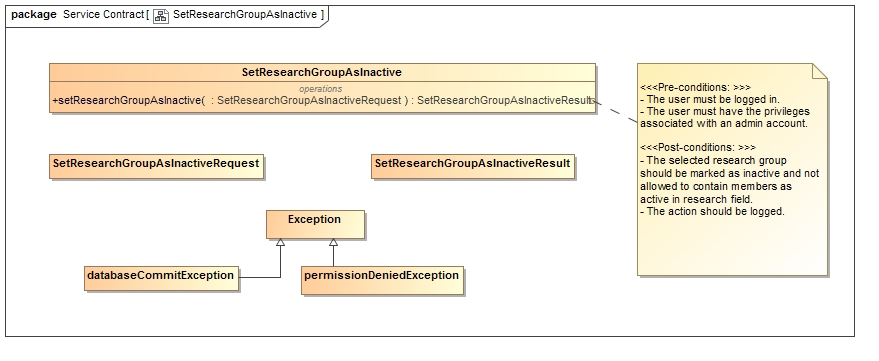
\includegraphics[width=\linewidth]{../Diagrams/ServiceContracts/Group control subsystem/SetResearchGroupAsInactive.jpg}
							\caption{Service Contract - Set Research Group as Inactive}
						\end{figure}
					\end{itemize}

					\cleardoublepage
					\item \textbf{Edit Any Research Group's Information} \hfill \textit{Priority: Critical}
					\begin{itemize}
						\item An admin user should be able to edit the information associated with any of the research groups within the system.
						\item \textbf{Pre-conditions:}
						\begin{itemize}
							\item The user must be logged in.
							\item The user must have the privileges associated with an admin user.
						\end{itemize}
						\item \textbf{Post-conditions:}
						\begin{itemize}
							\item The information associated with the particular research group should have been updated within the system.
							\item This action should be logged.
						\end{itemize}
						\item \textbf{Request and Results Data Structures:}
						\begin{figure}[H]
							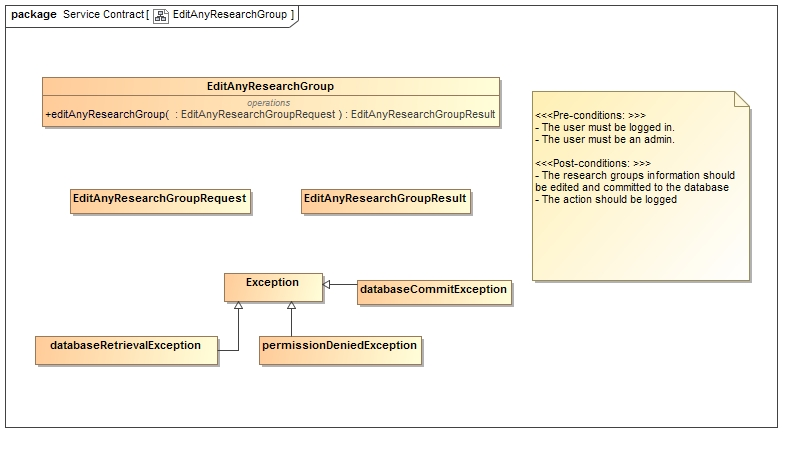
\includegraphics[width=\linewidth]{../Diagrams/ServiceContracts/Group control subsystem/EditAnyResearchGroup.jpg}
							\caption{Service Contract - Edit Any Research Group}
						\end{figure}
					\end{itemize}

					\cleardoublepage
					\item \textbf{Allocate/Change Head of Research Group} \hfill \textit{Priority: Critical}
					\begin{itemize}
						\item An admin user should be able to allocate a registered user to be the head of a particular research group, in turn allowing for this user to have more privileges within the system. An admin user should also be able to change the head of a research group.
						\item \textbf{Pre-conditions:}
						\begin{itemize}
							\item The user must be logged in.
							\item The user must have the privileges associated with an admin user.
						\end{itemize}
						\item \textbf{Post-conditions:}
						\begin{itemize}
							\item In the case of allocating the allocated user should now have the necessary rights and privileges to manage and view their allocated research group.
							\item In the case of changing the old head of a research group should have their privileges removed and the new head should be granted those privileges.
							\item This action should be logged.
						\end{itemize}
						\item \textbf{Request and Results Data Structures:}
						\begin{figure}[H]
							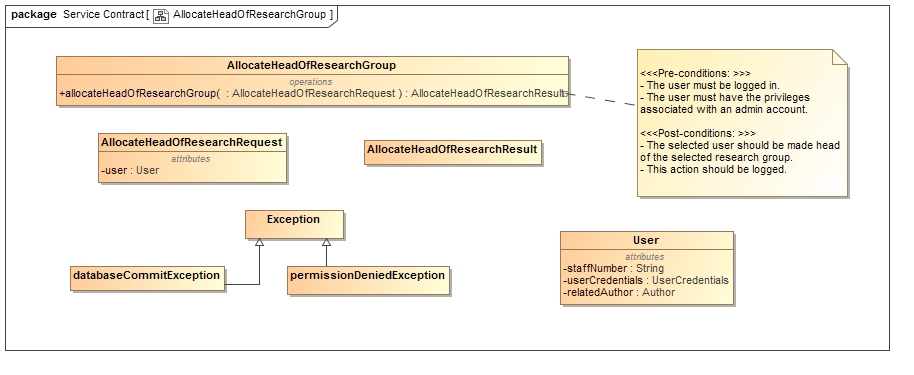
\includegraphics[width=\linewidth]{../Diagrams/ServiceContracts/Group control subsystem/AllocateHeadOfResearchGroup.jpg}
							\caption{Service Contract - Allocate Head of Research Group}
						\end{figure}
					\end{itemize}
				\end{itemize}
				
				\cleardoublepage
				\subsubsection{Logging Sub-System}\label{subsubsec:logging}
				Handles the logging of all important interactions which take place on the system.\\
				[3mm]
				\textbf{Admin:}
				\begin{itemize}
					\item \textbf{Download and View Log Text Files} \hfill \textit{Priority: Critical}
					\begin{itemize}
						\item An admin user should be able to download a text file containing the logs of the system.
						\item \textbf{Pre-conditions:}
						\begin{itemize}
							\item The user must be logged in.
							\item The user must have the privileges associated with an admin.
						\end{itemize}
						\item \textbf{Post-conditions:}
						\begin{itemize}
							\item A file should be made available to download containing all the relevant logs which the admin requested.
						\end{itemize}
						\item \textbf{Request and Results Data Structures:}
						\begin{figure}[H]
							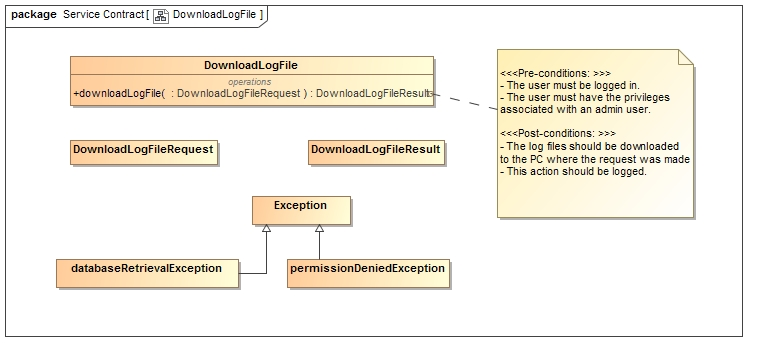
\includegraphics[width=\linewidth]{../Diagrams/ServiceContracts/Logging subsystem/DownloadLogFile.jpg}
							\caption{Service Contract - Download Log File}
						\end{figure}
					\end{itemize}
				\end{itemize}
				\textbf{Date and Time:}
				\begin{itemize}
					\item \textbf{Move Current Log File to Backup} \hfill \textit{Priority: Important}
					\begin{itemize}
						\item The system should periodically backup the current log file.
						\item \textbf{Pre-conditions:}
						\begin{itemize}
							\item A certain period of time must have passed.
						\end{itemize}
						\item \textbf{Post-conditions:}
						\begin{itemize}
							\item The old log file should have been backed up.
							\item A new log file should be created.
						\end{itemize}
						\item \textbf{Request and Results Data Structures:}
						\begin{figure}[H]
							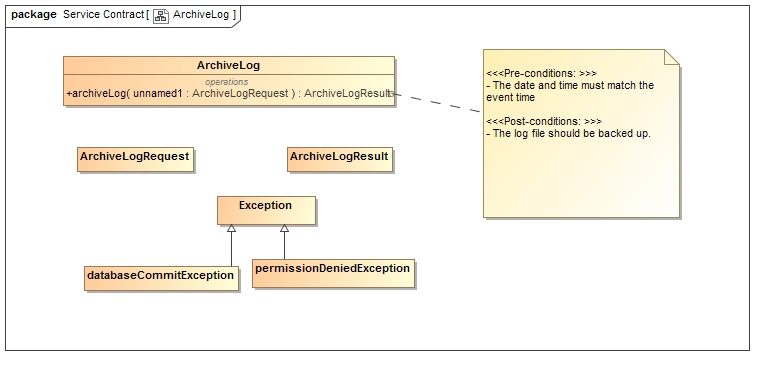
\includegraphics[width=\linewidth]{../Diagrams/ServiceContracts/Logging subsystem/ArchiveLog.jpg}
							\caption{Service Contract - Archive Log}
						\end{figure}
					\end{itemize}
					
					\item \textbf{Create New Log File} \hfill \textit{Priority: Important}
					\begin{itemize}
						\item After backing up the previous log file a new one should be created in order to replace the previous one.
						\item \textbf{Pre-conditions:}
						\begin{itemize}
							\item The old log file must have been backed up.
						\end{itemize}
						\item \textbf{Post-conditions:}
						\begin{itemize}
							\item A new log file should replace the older log file so that it can record any future logs.
						\end{itemize}
						\item \textbf{Request and Results Data Structures:}
					\end{itemize}
				\end{itemize}
			
		\cleardoublepage
		\subsection{Required Functionality}\label{subsec:requiredfunctionionality}
			\subsubsection{Publication Sub-System}
			\begin{figure}[H]
				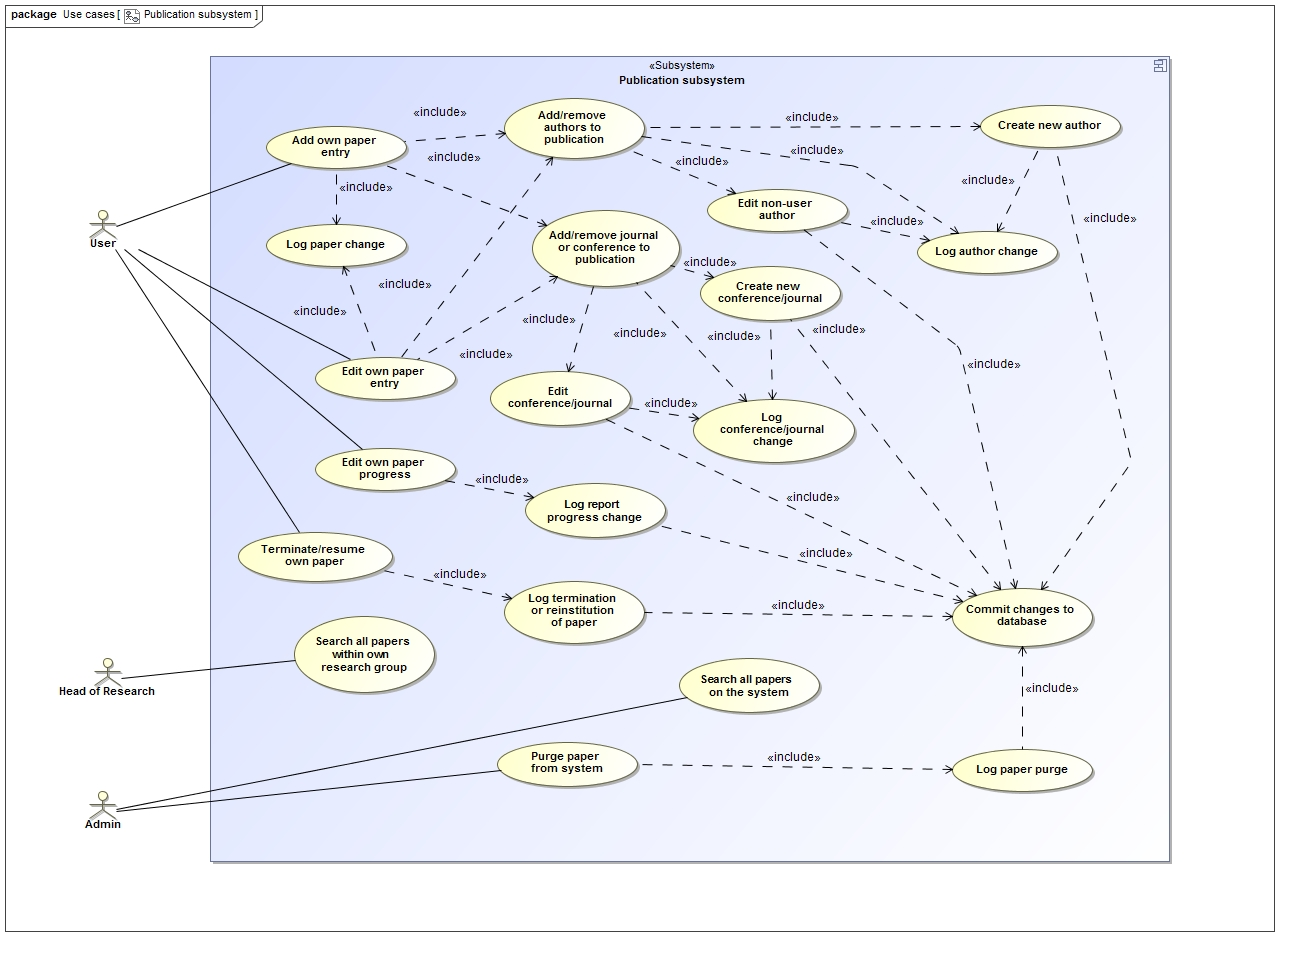
\includegraphics[width=\linewidth]{../Diagrams/Use Cases/Publication subsystem.jpg}
				\caption{Use Case - Publication Sub-System}
			\end{figure}
			
			\cleardoublepage
			\subsubsection{User Sub-System}
			\begin{figure}[H]
				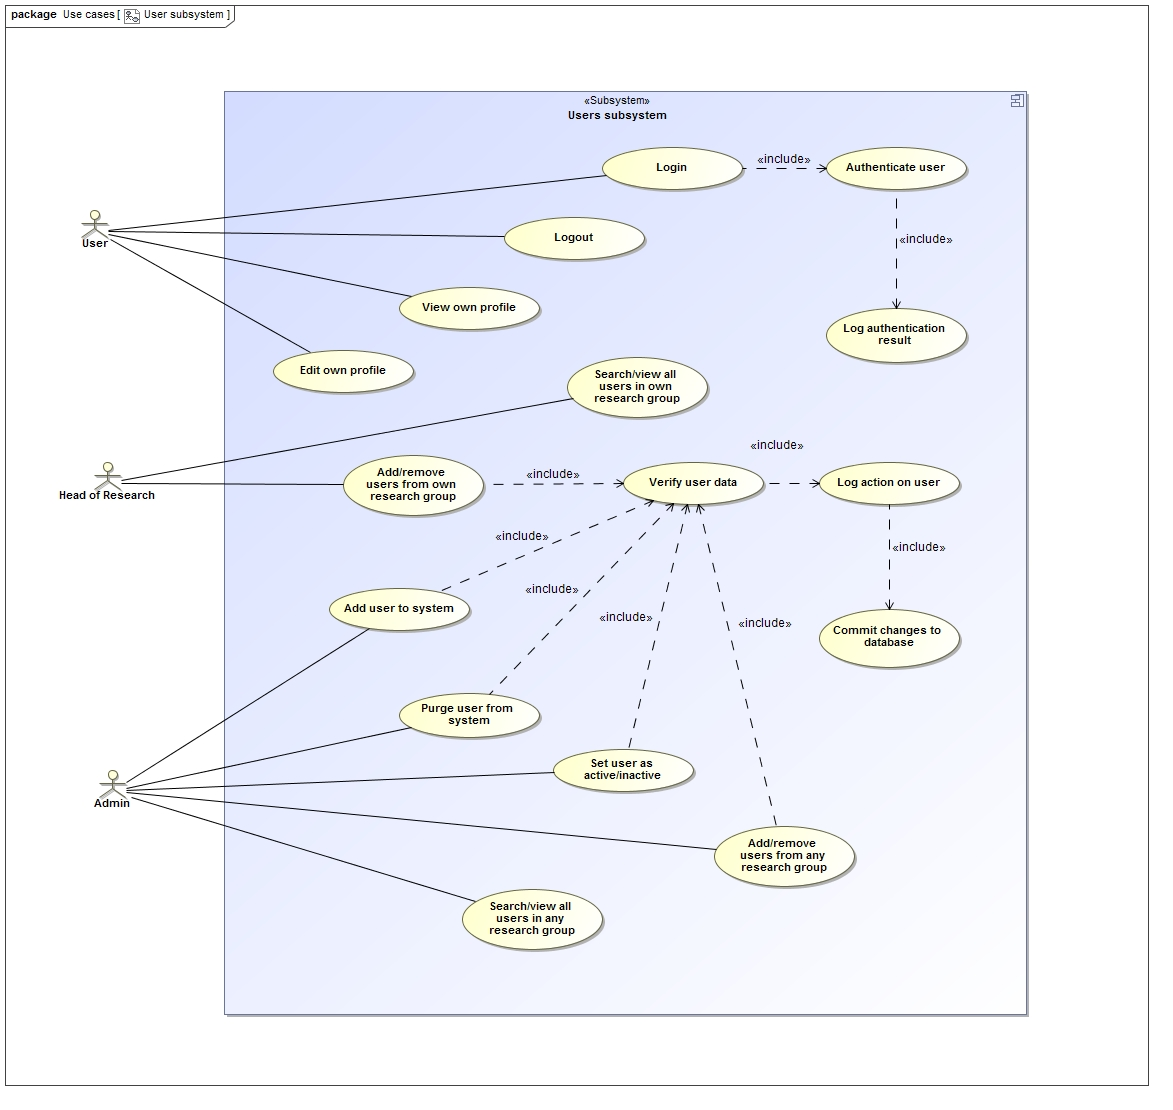
\includegraphics[width=\linewidth]{../Diagrams/Use Cases/User subsystem.jpg}
				\caption{Use Case - User Sub-System}
			\end{figure}
			
			\cleardoublepage
			\subsubsection{Notification Sub-System}
			\begin{figure}[H]
				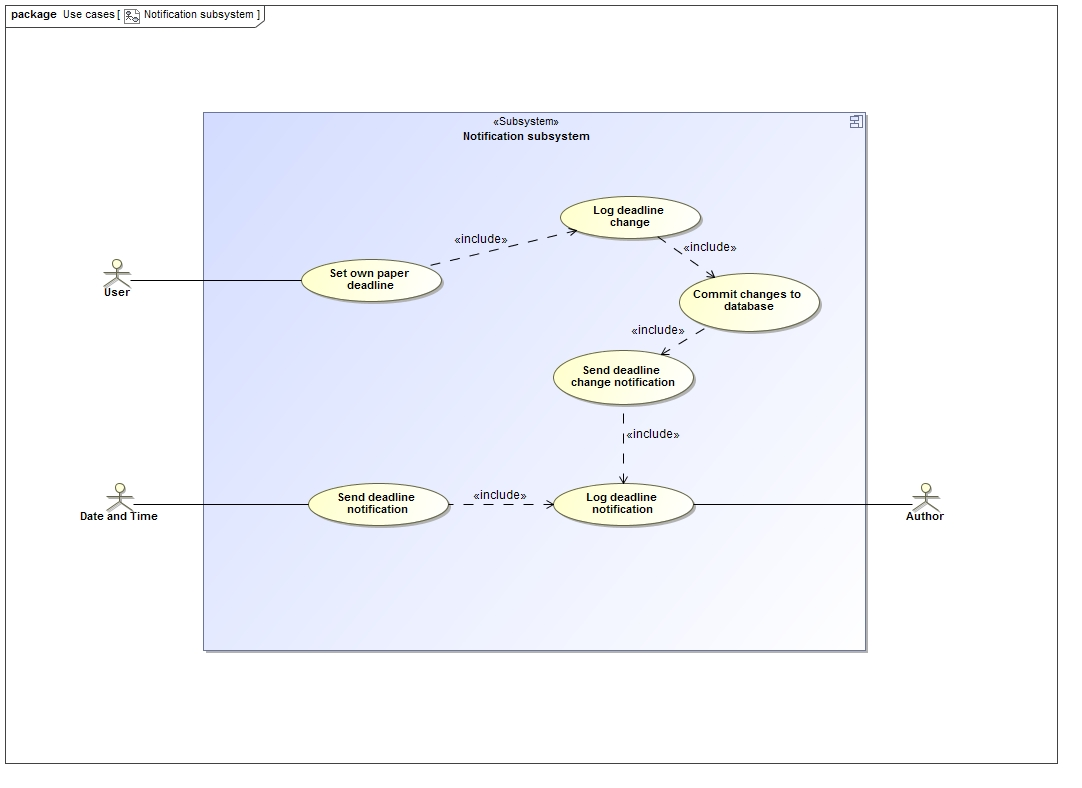
\includegraphics[width=\linewidth]{../Diagrams/Use Cases/Notification subsystem.jpg}
				\caption{Use Case - Notification Sub-System}
			\end{figure}
			
			\cleardoublepage
			\subsubsection{Reporting Sub-System}
			\begin{figure}[H]
				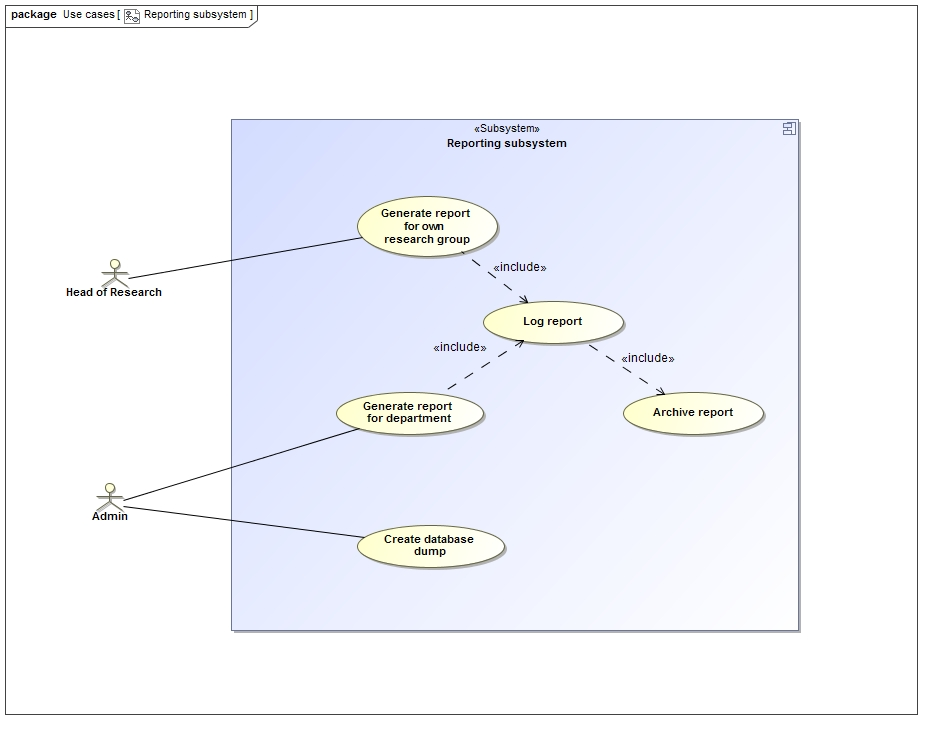
\includegraphics[width=\linewidth]{../Diagrams/Use Cases/Reporting subsystem.jpg}
				\caption{Use Case - Reporting Sub-System}
			\end{figure}	
			
			\cleardoublepage
			\subsubsection{Group Control Sub-System}
			\begin{figure}[H]
				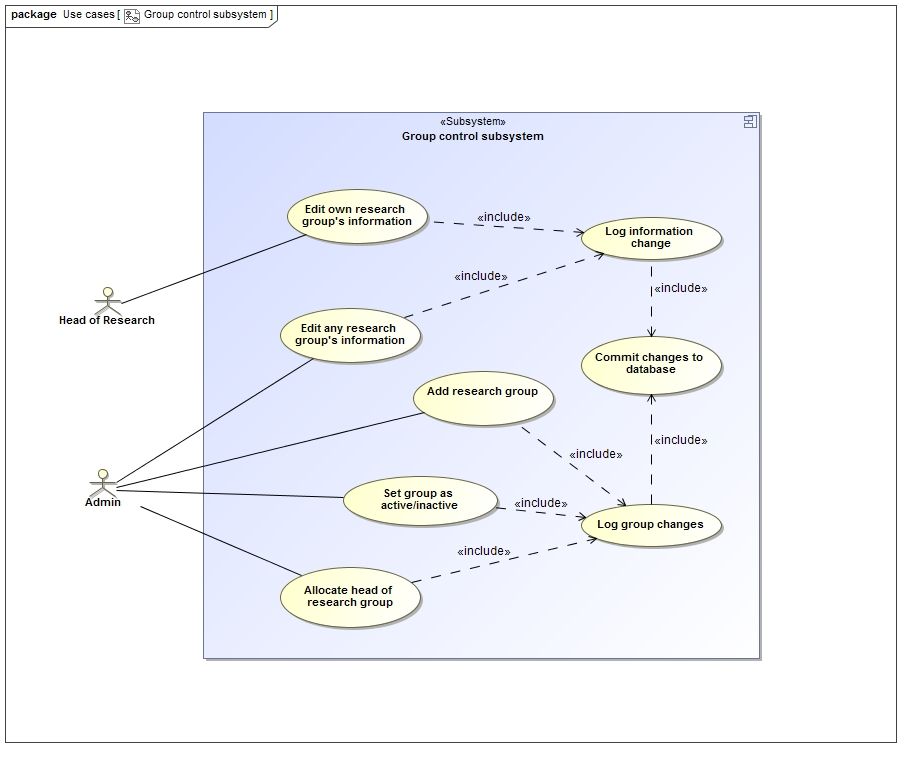
\includegraphics[width=\linewidth]{../Diagrams/Use Cases/Group control subsystem.jpg}
				\caption{Use Case - Group Control Sub-System}
			\end{figure}
			
			\cleardoublepage
			\subsubsection{Logging Sub-System}
			\begin{figure}[H]
				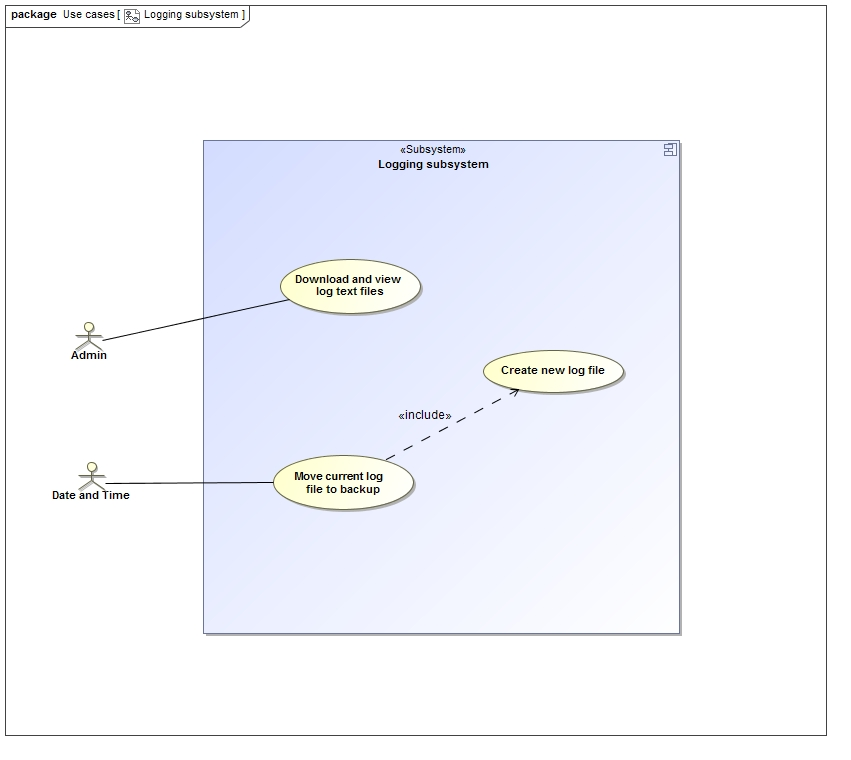
\includegraphics[width=\linewidth]{../Diagrams/Use Cases/Logging subsystem.jpg}
				\caption{Use Case - Logging Sub-System}
			\end{figure}
			
		\cleardoublepage	

		\subsection{Process Specifications}\label{subsec:processspecification}
		Certain use cases require further information with regards to their function.\\ These use cases are specified further by means of process specification.
		\subsubsection{Publication Sub-System}
			\begin{figure}[H]
				\includegraphics[width=4in, center]{../Diagrams/Process Specifications/Publication subsystem/Add_Edit Own Paper Entry.jpg}
				\caption{User - Add/Edit Own Paper Entry}
			\end{figure}
			\begin{figure}[H]
				\includegraphics[width=4in, center]{../Diagrams/Process Specifications/Publication subsystem/Edit Own Paper Progress.jpg}
				\caption{User - Edit Own Paper Progress}
			\end{figure}
			\begin{figure}[H]
					\includegraphics[width=4in, center]{../Diagrams/Process Specifications/Publication subsystem/Terminate_Resume Own Paper.jpg}
					\caption{User - Terminate/Resume Own Paper}
			\end{figure}
			\begin{figure}[H]
				\includegraphics[width=4in, center]{../Diagrams/Process Specifications/Publication subsystem/Add_Remove Authors from a paper.jpg}
				\caption{User - Add/Remove Authors From a Paper}
			\end{figure}
			\begin{figure}[H]
				\includegraphics[width=4in, center]{../Diagrams/Process Specifications/Publication subsystem/Add_Remove PublicationType From Paper.jpg}
				\caption{User - Add/Remove PublicationType From Paper}
			\end{figure}
			\begin{figure}[H]
				\includegraphics[width=4in, center]{../Diagrams/Process Specifications/Publication subsystem/Add_Edit Author.jpg}
				\caption{User - Add/Edit Author}
			\end{figure}
			\begin{figure}[H]
				\includegraphics[width=4in, center]{../Diagrams/Process Specifications/Publication subsystem/Add_Edit PublicationType.jpg}
				\caption{User - Add/Edit PublicationType}
			\end{figure}
			\begin{figure}[H]
				\includegraphics[width=4in, center]{../Diagrams/Process Specifications/Publication subsystem/Search All Papers.jpg}
				\caption{Head of Research/Admin - Search All Papers}
			\end{figure}
			\begin{figure}[H]
				\includegraphics[width=4in, center]{../Diagrams/Process Specifications/Publication subsystem/Purge Paper.jpg}
				\caption{Admin - Purge Paper}
			\end{figure}	
		\subsubsection{User Sub-System}
			\begin{figure}[H]
				\includegraphics[width=4in, center]{../Diagrams/Process Specifications/User subsystem/Login.jpg}
				\caption{User - Login}
			\end{figure}
			\begin{figure}[H]
				\includegraphics[width=4in, center]{../Diagrams/Process Specifications/User subsystem/Logout.jpg}
				\caption{User - Logout}
			\end{figure}
			\begin{figure}[H]
				\includegraphics[width=4in, center]{../Diagrams/Process Specifications/User subsystem/View Own Profile.jpg}
				\caption{User - View Own Profile}
			\end{figure}
			\begin{figure}[H]
				\includegraphics[width=4in, center]{../Diagrams/Process Specifications/User subsystem/Edit Own Profile.jpg}
				\caption{User - Edit Own Profile}
			\end{figure}
			\begin{figure}[H]
				\includegraphics[width=4in, center]{../Diagrams/Process Specifications/User subsystem/Add_Remove Users from Research Group.jpg}
				\caption{Head of Research - Add/Remove All Users in a Research Group}
			\end{figure}
			\begin{figure}[H]
				\includegraphics[width=4in, center]{../Diagrams/Process Specifications/User subsystem/Add New User.jpg}
				\caption{Admin - Add New User to System}
			\end{figure}
			\begin{figure}[H]
				\includegraphics[width=4in, center]{../Diagrams/Process Specifications/User subsystem/Purge User From System.jpg}
				\caption{Admin - Purge User from System}
			\end{figure}
			\begin{figure}[H]
				\includegraphics[width=4in, center]{../Diagrams/Process Specifications/User subsystem/Set User as Active_Inactive.jpg}
				\caption{Admin - Set User as Active or Inactive}
			\end{figure}
			\begin{figure}[H]
				\includegraphics[width=4in, center]{../Diagrams/Process Specifications/User subsystem/Add_Remove User from any Research Group.jpg}
				\caption{Admin - Add/Remove Users from any Research Group}
			\end{figure}
			\begin{figure}[H]
				\includegraphics[width=4in, center]{../Diagrams/Process Specifications/User subsystem/View All User Profiles.jpg}
				\caption{Admin - Search/View All Users in any Research Group}
			\end{figure}
			
			\subsubsection{Notification Sub-System}
			\begin{figure}[H]
				\includegraphics[width=4in, center]{../Diagrams/Process Specifications/Notification subsystem/Set Paper Deadline.jpg}
				\caption{User - Set Paper Deadline}
			\end{figure}
			\begin{figure}[H]
				\includegraphics[width=4in, center]{../Diagrams/Process Specifications//Notification subsystem/Send Deadline Notification.jpg}
				\caption{System - Send Deadline Notification}
			\end{figure}
			\begin{figure}[H]
				\includegraphics[width=4in, center]{../Diagrams/Process Specifications//Notification subsystem/Send Deadline Update Notification.jpg}
				\caption{System - Send Deadline Update Notification}
			\end{figure}

			\subsubsection{Reporting Sub-System}
			\begin{figure}[H]
				\includegraphics[width=4in, center]{../Diagrams/Process Specifications/Reporting subsystem/Generate Report for Research Group.jpg}
				\caption{Head of Research - Generate Report for Research Group}
			\end{figure}
			\begin{figure}[H]
				\includegraphics[width=4in, center]{../Diagrams/Process Specifications/Reporting subsystem/Generate Report for Department.jpg}
				\caption{Admin - Generate Report for Department}
			\end{figure}
			\begin{figure}[H]
				\includegraphics[width=4in, center]{../Diagrams/Process Specifications/Reporting subsystem/Dump Database to File.jpg}
				\caption{Admin - Dump Database to File}
			\end{figure}
			
			\subsubsection{Group Control Sub-System}
				\begin{figure}[H]
				\includegraphics[width=4in, center]{../Diagrams/Process Specifications/Group control subsystem/Add Research Group.jpg}
				\caption{Admin - Add Research Group}
			\end{figure}
			\subsubsection{Logging Sub-System}
				\begin{figure}[H]
					\includegraphics[width=4in, center]{../Diagrams/Process Specifications/Logging subsystem/Archive Logs.jpg}
					\caption{DateTime - Archive Logs}
				\end{figure}
				\begin{figure}[H]
					\includegraphics[width=4in, center]{../Diagrams/Process Specifications/Logging subsystem/Download log files.jpg}
					\caption{Admin - Download Log Files}
				\end{figure}
			
		\cleardoublepage
		\subsection{Domain Model}\label{subsec:domainmodel}
		The domain model is described in terms of class diagram.\\ Class diagrams contain information on the current class such as attributes and relationships to other classes.
		
			\begin{figure}[H]				
				\includegraphics[width=\linewidth]{../Diagrams/Domain Model/domainModel.jpg}
				\caption{ Domain model - Classes related to each domain }
			\end{figure}
			\begin{center}
			\textbf{Domains include :}
			\end{center}
		\begin{multicols}{2}
		
			\begin{itemize} 
				\item \textbf{User Domain:}
						\begin{itemize}
						\item User
						\item UserCredentials
						\item Author
						\end{itemize}
					
				\item \textbf{Logging Domain:}
						\begin{itemize}
						\item LogHandler
						\item LogFile
						\end{itemize}				
					
					
				\item \textbf{Group Control Domain:}
						\begin{itemize}
						\item ResearchGroup
						\end{itemize}
						
					\columnbreak

					
				\item \textbf{Reports Domain:}

						\begin{itemize}
						\item ReportGenerator
						\item Report
						\end{itemize}
					
				\item \textbf{Notifications Domain:}
						\begin{itemize}
						\item NotificationHandler
						\item Notification
						\end{itemize}

					
				\item \textbf{Publication Domain:}
						\begin{itemize}
						\item Publication
						\item PublicationType
						\item Conference
						\item Journal
						\end{itemize}		
				
			\end{itemize}
		\end{multicols}
	\cleardoublepage
	\section{Open Issues}\label{sec:issues}
	Issues that weren't discussed in the client requirements meeting:
		\begin{itemize}
		  \item 
		  \item 
		\end{itemize}
		
\end{document}
